%  Kandidate prosimo, da nam posredujejo predloge za izbolj''save tega vzorca 
%  na elektronski naslov Fizikalne knji''znice: fiz.knjiz@fmf.uni-lj.si.
%---------------------------------------------------------------------------------------
%        METAPODATKI
%--------------------------------------------------------------------------------------

\begin{filecontents*}{\jobname.xmpdata}
\Title{Naslov doktorske disertacije v angleškem jeziku}
\Author{Klemen Čotar}
\Keywords{disertacije\sep navodila}
\Subject{Physics}
\end{filecontents*}

%--------------------------------------------------------------------------------------

\documentclass[longbibliography,english,a4paper,12pt]{book}

\usepackage[english]{babel}    
\usepackage[utf8]{inputenc}
\usepackage{amsfonts}
\usepackage[T1]{fontenc}
\usepackage[pdftex]{graphicx}
\usepackage{fancyhdr}
\usepackage[sort, numbers]{natbib}
\usepackage{acro}

%--------------------------------------------------------------------------------------
%      DEFINICIJA AKRONIMOV
%--------------------------------------------------------------------------------------


\DeclareAcronym{FMF}{
  short            = FMF,
  long             = Fakulteta za matematiko in fiziko,
  class		= abbrev
  }

  
%-----------------------------------------------------------------------------------
%     PDF/A
%----------------------------------------------------------------------------------

\usepackage{xmpincl}
%\usepackage[a-1b]{pdfx} 

%------------------------------------------------------------------------------------  

\usepackage{filecontents}
\usepackage{hyperref}
\usepackage{url}
\usepackage[a4paper,inner=3.5cm,outer=2.5cm,top=2.5cm,bottom=2.5cm,pdftex]{geometry}
\usepackage[titletoc,title]{appendix}
\usepackage{epstopdf}
\usepackage{makeidx}
\pagestyle{fancy}
\setlength{\headheight}{15pt}
\usepackage{enumitem}
\usepackage{underscore}
\usepackage{tocloft}
\renewcommand{\cftpartleader}{\cftdotfill{\cftdotsep}} 
\renewcommand{\cftchapleader}{\cftdotfill{\cftdotsep}} 

\makeindex

\def\epsfg#1#2{\epsfig{file=#1.eps,width=#2}}
\def\legendamp#1#2{\vbox{\hsize=#1\caption{\small #2}}}

\setcounter{topnumber}{4}
\setcounter{bottomnumber}{4}
\setcounter{totalnumber}{5}
\renewcommand{\topfraction}{0.99}
\renewcommand{\bottomfraction}{0.99}
\renewcommand{\textfraction}{0.0}
\setlength{\tabcolsep}{10pt}
\renewcommand{\arraystretch}{1.5}

\def\bi#1{\hbox{\boldmath{$#1$}}}
\let\oldvec\vec
\def\vec#1{\mbox{\boldmath$#1$}}
\def\pol{{\textstyle{1\over2}}}
\def\svec#1{\mbox{{\scriptsize \boldmath$#1$}}}

%----------------------------------------------------------------------------------------
%    SUMNIKI
%----------------------------------------------------------------------------------------
%  Za pisanje sumnikov imamo tri moznosti:
%   --- vnasamo jih neposredno v kodnem sistemu UTF-8 (priporocljivo)
%   --- pisemo jih z latexovim ukazom, ki je namenjen natanko temu,
%       in sicer kot \v{c}, \v{s}, \v{z}, \v{C}, \v{S}, v{\Z} ali
%       malo manj pregledno kot \v c, \v s, \v z, \v C, \v S, \v Z,


%------------------------------------------------------------------------------------------
%   PRIPOROCILO
%
%  V primeru, da je besedilna datoteka prevelika za pregledno urejanje,
%  priporocamo, da vsebino razdelite na posamezna poglavja, ki jih v glavni
%  dokument vkljucite z ukazom \input{naslov_poglavja}.
%
%------------------------------------------------------------------------------------------

\begin{document}

%-----------------------------------------------------------------------------------------
%       NASLOVNA STRAN V ANGLESKEM JEZIKU
%----------------------------------------------------------------------------------------

\pagestyle{empty}
\begin{center}

{\large UNIVERSITY OF LJUBLJANA\\
FACULTY OF MATHEMATICS AND PHYSICS\\
DEPARTMENT OF PHYSICS\\}

\vspace{4cm}

{\Large Klemen Čotar\\}

\vspace{10mm}

{\bf \Large NASLOV DOKTORSKE DISERTACIJE V ANGLEŠKEM JEZIKU}\\
\vspace{5mm}
{\sc Doctoral thesis}\\

\vfill

{\large ADVISER: prof. dr. Tomaž Zwitter\\

\vspace{2cm}
Ljubljana, 2020}

\end{center}

%------------------------------------------------------------------------------------------------
%       NASLOVNA STRAN V SLOVENSKEM JEZIKU
%-----------------------------------------------------------------------------------------------

\cleardoublepage
\begin{center}

{\large UNIVERZA V LJUBLJANI\\
FAKULTETA ZA MATEMATIKO IN FIZIKO\\
ODDELEK ZA FIZIKO\\}

\vspace{4cm}

{\Large Klemen Čotar\\}

\vspace{10mm}

{\bf \Large NASLOV DOKTORSKE DISERTACIJE V SLOVENSKEM JEZIKU}\\
\vspace{5mm}
{\sc Doktorska disertacija}\\

\vfill

{\large MENTOR: prof. dr. Tomaž Zwitter\\

\vspace{2cm}
Ljubljana, 2020}

\end{center}
%------------------------------------------------------------------------------------------------
%        ZAHVALA (NEOBVEZNO)
%------------------------------------------------------------------------------------------------

\cleardoublepage
\mbox{}
\vfill
\foreignlanguage{slovene}{
{\Large \bf Zahvala}
\vspace{1cm}\\
Na tem mestu zapišite, komu se zahvaljujete za pomoč pri nastanku doktorske disertacije.
}

%-----------------------------------------------------------------------------------------------
%         IZVLECEK
%----------------------------------------------------------------------------------------------

\cleardoublepage
\foreignlanguage{slovene}{  % slovenski delilni vzorci
\begin{center}
{\bf Naslov v slovenskem jeziku}\\[3mm]
{\sc  Izvleček}
\end{center}
\vspace{10mm}
Kratek izvleček v slovenskem jeziku, do 300 besed.\\[10mm]
{\bf Ključne besede:}\\[3mm]
{\bf PACS:}
}


\cleardoublepage
\begin{center}
{\bf Naslov v angleškem jeziku}\\[3mm]
{\sc  Abstract}
\end{center}
\vspace{10mm}
Kratek izvleček v angleškem jeziku, do 300 besed.\\[10mm]
{\bf Keywords:}\\[3mm]
{\bf PACS:}

%---------------------------------------------------------------------------------------------------
%    KAZALO
%---------------------------------------------------------------------------------------------------

\cleardoublepage
\tableofcontents

%--------------------------------------------------------------------------------------------------
%        SEZNAM SLIK (NEOBVEZNO)
%---------------------------------------------------------------------------------------------------

%\cleardoublepage\phantomsection
%\renewcommand\listfigurename{List of figures}
%\addcontentsline{toc}{chapter}{\listfigurename}
%\listoffigures

%---------------------------------------------------------------------------------------------------
%        SEZNAM TABEL (NEOBVEZNO)
%---------------------------------------------------------------------------------------------------

%\cleardoublepage\phantomsection
%\renewcommand\listtablename{List of tables}
%\addcontentsline{toc}{chapter}{\listtablename}
%\listoftables

%--------------------------------------------------------------------------------------------------
%        SEZNAM KRATIC, SEZNAM SIMBOLOV (NEOBVEZNO)
%------------------------------------------------------------------------------------------------

%\cleardoublepage\phantomsection
%\chapter*{List of abbreviations and symbols}
%\renewcommand\listtablename{List of abbreviations and symbols}
%\addcontentsline{toc}{chapter}{\listtablename}
%\printacronyms[include-classes=abbrev, name=Abbreviations]
%\printacronyms[include-classes=nomencl, name=Symbols]
%\cleardoublepage

%--------------------------------------------------------------------------------------------------
%       OSREDNJI DEL
%--------------------------------------------------------------------------------------------------

\pagestyle{fancy}
\fancyhead[CE,RE]{}
\fancyhead[LO,CO]{}
\fancyhead[LE]{\textbf{\nouppercase{\leftmark}}}
\fancyhead[RO]{\textbf{\nouppercase{\rightmark}}}


\chapter{Introduction}
Primeri citiranj:

citealp: \citealp{APS}

citealp*: \citealp*{APS}

citealt: \citealt{APS}

citealt*: \citealt*{APS}

citeauthor: \citeauthor{APS}

citeauthor*: \citeauthor*{APS}

citefullauthor: \citefullauthor{APS}

citeauthor*: \citeauthor*{APS}

citenum: \citenum{APS}

citep: \citep{APS}

citet: \citet{APS}

citet*: \citet*{APS}

citeyear: \citeyear{APS}

citeyearpar: \citeyearpar{APS}

 % intro
Observational studies and simulations show that stars in our Galaxy were not formed at the same time, but at multiple epochs in different places of the Galaxy \cite{2001ApJ...554.1044C, 2017ARA&A..55...59N}. One of the youngest building blocks of the Galaxy are open stellar clusters whose stars formed from the same molecular cloud of material \cite{2003ARA&A..41...57L} and therefore retain some properties of the original cloud they were made from. Stellar properties of an individual star can be separated into a kinematic and chemical component. The first is describing the position and movement of a star in the Galaxy. The second gives information about its chemical composition and physical properties. During the evolution of the Galaxy, clusters that have a lower number of members and are therefore gravitationally loosely bound, slowly evaporate because of different effects such as gravitational dynamical friction and ejection of stars during close intra-cluster stellar interactions. The latter is a result of close gravitational interactions among members, where one of them can be ejected out of a cluster at high velocity \cite{2009MNRAS.396..570G, 2010MNRAS.402..105G, 2017MNRAS.470.3049R}. Such past members can on the sky be found even several degrees away from their main cluster body \cite{2007MNRAS.376L..29G, 2018MNRAS.473.4612K, 2019ApJ...884....6M}. The gravitational dynamical friction happens when a cluster moves trough regions of the Galaxy with a higher density of stars \cite{2010MNRAS.401.2753B}. During such event, the gravity of a cluster starts pulling seemingly fixed stars around it. Considering energy and momentum conservation law, we can conclude that a cluster will be slowed down for the same amount. This slowing subsequently changes the orbit of individual cluster members around the centre of the Galaxy. Small orbital changes lead to a gradual expansion of a cluster volume that can be tracked until its individual stars blend with a general stellar field population, making them unrecognizable as past cluster members. The most prominent transitional features we can observe are compact cluster tidal tails \cite{2019AA...627A...4R, 2019AJ....157..115Y, 2019AA...621L...3M, 2019arXiv191206657Z} and lose extended halos of evaporated stars. The halos can be observed as a slowly decreasing over-density \cite{2002A&A...385..471C, 2004A&A...427..485B, 2019AA...627A.119C} of stars far from a denser central cluster core.

% cluster ages
Born from the same molecular cloud, open clusters are therefore ideal tracers of formation, assembly and evolutionary history of their host galaxies. Being influenced by external and internal processes, their lifetime is limited from about $100$~Myr to a few Gyr for the densest structures \cite{1998A&A...337..363P, 2013MNRAS.434.2509M}. Studies have shown that the dissolution time of a cluster depends mainly on its total mass, its radius and its galactic environment (density of the stars around it and on its galactic path). Many papers have so far dealt with the question of determining the precise lifetime of stellar clusters before they completely dissipate into field population. The problem has been tackled using direct N-body simulations \cite{1998A&A...337..363P} where the movement of individual stars was traced, and from direct observational data \cite{1971Ap&SS..13..300W, 1988IAUS..126..393W, 2019MNRAS.487.2385M, 2019A&A...623A.108B} using isochrone fits. Age distribution of open clusters within a distance of $1$~kpc from the Sun shows a cluster median lifetime of $200$~Myr. Their broad range in ages gives us a possibility of observing them at different evolutionary stages \cite{2006BASI...34..153C, 2007A&A...468..139P} before they blend \cite{2001A&A...366..827B} into a field stellar population. On the other hand, such a short lifetime (in comparison with a lifetime of a Sun-like star) gives us a limited number of bounded clusters in the sky that can be studied at a given time.

% imf and mass segregation
The processes described above heavily depend on the mass of a cluster, its internal structure and mass distribution of its components. When star formation ceases, we are left with a wide range of stellar masses. Their distribution can be described by an initial mass function (IMF) \cite{1955ApJ...121..161S, 1986FCPh...11....1S, 2003PASP..115..763C} that appears invariant among clusters and even stars in the field \cite{2001MNRAS.322..231K}. The initial spatial distribution of stars in young clusters may reflect the structure of parental molecular cloud \cite{2015MNRAS.448.1847H}. In many stellar clusters, the brightest and most massive stars are concentrated towards the centre of a cluster, this state is usually attributed to mass segregation. Whether mass segregation occurs due to an evolutionary effect or it is of primordial origin is not yet entirely clear \cite{1998A&A...333..897R, 1998MNRAS.295..691B, 2002MNRAS.331..245D, 2003A&A...405..525B}. In the first case, massive stars are formed all around the cluster volume and eventually sink to its centre through the effect of two-body relaxations. In the second scenario, massive stars form preferentially in the central region of a cluster either by gas accretion due to their favourable location at the bottom of a gravitational potential well or through a coalescence process of less massive stars. The fact that mass segregation is also observed in young clusters might suggest that the second scenario is more likely that the evolutionary mass segregation, but the question is still under investigation \cite{2018MNRAS.473..849D}.

% binaries 
Similarly to the IMF, we can also define the initial binary population (IBP) of the observed sample of stars. Characterizing fraction of binaries in stellar clusters is of great importance for many fields of astrophysics. Since binaries are on average more massive than single stars, they are thought to be useful tracers of dynamical mass segregation \cite{2015arXiv151000099D}. Comparing observations with a theoretical model for the radial distribution of binary systems and their properties (mass and luminosity ratio, orbital period) distribution can be used to assess the dynamical state of a cluster \cite{1999NewA....4..495K}.

\section{Open clusters in the \G\ era}
\label{sec:open_clust_gaia}
Since \G\ Data Processing and Analysis Consortium (DPAC) centres responsible for analysis of the \G\ observations started publishing publicly available ready-to-use stellar properties, many new discovers and insights have been made. For the first time in history, we reliably know the position, distance, complete spatial velocity (proper motion and radial velocity) and luminosity for millions of bright and dim stars all across the observable sky. Their accuracy heavily depends on the source brightness. For example, published \G\ parallax uncertainties are in the range from $0.04$ to $0.7$~mas for the faintest sources. Similarly, radial velocities are precisely known in the range from 300~\ms to 3~\kms (further details are given in Section \ref{sec:gaia_data}).

One of the fields in astronomy that massively benefited from those new and improved measurements was a research of open stellar clusters.

% looking for clusters, unreliable detection
A traditional historical way to look for open stellar clusters was through counting stars as they are seen on the sky from Earths' location and finding over-densities in those counts \cite{1988AJ.....95..108L, 2014A&A...568A..51S}. To perform a more robust selection, members were additionally filtered based on their apparent distance from the cluster centre and their motion vectors \cite{2017A&A...601A..19G}. Using the latest second release of \G\ data \citep[DR2,][]{2018A&A...616A...1G}, we can go beyond that and build upon the results achieved by the methods mentioned above. Complete \G\ information on stellar distance, kinematics and photometric measurements enable us to go beyond simple methodologies, to unravel even the faintest and sparsest components of open clusters. So far, many works have been published trying to refine parameters, and membership information of long known open clusters \cite{2017A&A...601A..19G, 2018A&A...618A..93C, 2019A&A...627A..35C} and find new, less numerous or fainter clusters \cite{2019arXiv190904612B, 2019ApJS..245...32L, 2019JKAS...52..145S, 2019A&A...624A.126C, 2020arXiv200107122C}. Such thorough and the improved investigation uncovered that many of the clusters listed in modern catalogues, initially discovered as apparent stellar overdensities, are no more than chance alignments of stars and not true physically bound clusters \cite{1998A&A...340..402B, 2000A&A...357..145C, 2016AJ....152....7H, 2018MNRAS.480.5242K, 2020A&A...633A..99C}.

% starosti zvezd za kopice in field
Precisely determined open cluster membership also enables accurate age determination of a cluster and its stars \cite{2018ApJ...863...65C}. When observing stars in any random stellar field, it is notoriously hard to determine their ages as they remain unchanged for the majority of their lifetime. While it is possible to obtain precise age estimates for some specific classes of stars \cite{2010ARA&A..48..581S}, a uniform methodology does not exist for all. Age determination is much easier for stars in a cluster as they are all of a very similar age. Stellar evolution and its cycle are determined mainly by the initial mass of a star. Observing stars of different masses in a cluster reveals its evolutionary stage and consequently also its age by comparing them to theoretical evolutionary models. The latest \G\ data enabled researchers to compute stellar absolute magnitudes and colours that are commonly used in those comparisons \cite{2019MNRAS.487.2385M, 2019A&A...623A.108B, 2019A&A...631A.166K}.

% mass segregation
Another advantage of the newest \G\ dataset, with accurately determined distance to objects, is the possibility of determining the actual shape of a cluster, mass segregation of member stars and their gravitational potential from the first principles. Until recently that was possible only through n-body simulations \cite{1987MNRAS.224..193T, 2016MNRAS.456.3757S, 2018MNRAS.473..849D} that were compared with available observational datasets. For distant stellar associations, the distance error bars are still larger than a cluster itself, but improvements are expected when \G\ EDR3 will be released in the second half of the year 2020 or later. Internal cluster dynamics can in those cases be inferred using precisely determined radial velocities and proper motion vectors whose uncertainty is not affected by stellar distance, but their apparent brightness. Deviations (overtaking or lagging) from the mean cluster velocity can be therefore be used to assess in which direction, away from the mass centre, stars are moving. This velocity deviation consequently also indicates its position in a cluster. Reliable determination of stellar mass distribution in a cluster also depends on accurate classification of binary or higher multiplicity stars and their masses. By using pure \G\ information, they can be identified as stars with higher radial velocity uncertainty \cite{2018RNAAS...2b..20E}, by its temporal variation in future data releases \cite{2019AJ....158..155B}, using precise absolute magnitudes \cite{2018ApJ...857..114W, 2018A&A...616A..10G, 2019MNRAS.487.2474C} or by exploring astrometric uncertainties \cite{2020arXiv200305467B} that indicate movement of their combined photocentre. 

\section{Chemical tagging}
\label{sec:open_clustesr_tagging}
Majority of previously described works in Section \ref{sec:open_clust_gaia} relies on a complete 6D positional and kinematics information to discover clusters and their sub-structures. Advances in observational techniques and data analysis enables us to go beyond kinematics information and include a multidimensional chemical signature of stars -- the procedure known as chemical tagging \cite{2002ARA&A..40..487F, 2010ApJ...721..582B}. So far a blind chemical tagging (without kinematics) that would delineate between cluster and field stars has not yet been demonstrated with great success unless the observed structure has obviously different chemical composition \cite{2016ApJ...833..262H}. A trait that it is not common to open stellar clusters formed at about the same time \cite{2019A&A...629A..34G}, but to galactic components formed at vastly different epochs \cite{2018A&A...619A.125A} of Galaxy formation.

The measured chemical signature of a star gives us its composition in the outer-most layer, where it remains unchanged for young stars. Its composition is, therefore, a direct reflection of a medium from which it was built. Galaxy started evolving from dust made predominantly from hydrogen and helium which slowly got polluted by evolved stars during their final evolutionary stages. This gradual enrichment is nowadays observable as gradients of chemical abundances in radial and vertical directions of Galaxy. Internal gravitational mixing causes blending of those signatures as stars move to different orbits. Already complicated chemical structure of Galaxy is in some regions interrupted by newly created dense stellar structures -- open clusters -- which we would like to discover by the above-described procedure. Because of multiple gradual processes going on in Galaxy, the chemical tagging so far does not have clearly defined cuts to separate galactic components.

The latest research showed that many, even unexpected, observational and data reduction issues still have to be thoroughly investigated and resolved, especially if data from different surveys are to be combined \cite{2019ARA&A..57..571J}. Studies suggest that open clusters might not be as homogeneous as thought before \cite{2016ApJ...817...49B, 2018MNRAS.473.4612K}, and abundances show traits of stellar evolution \cite{2015A&A...577A..47B, 2017ApJ...840...99D, 2018MNRAS.478..425B}. On top of that, the main concerns of chemical tagging are abundance trends assumingly induced by spectral analysis \cite{2016ApJ...817...49B, 2019arXiv191208539C, 2020arXiv200103179B}. Observed trends depend on determined stellar physical parameters (i.e. \Teff\ and \vsin) and might be results of inadequate stellar models or actual stellar processes. To cope with this complexity and uncertainties, complex Bayesian models are being developed \cite{2016ApJ...817...49B, 2019ApJ...887...73C} in order to uncover and cluster abundance patterns. With this in mind, many work and validation still have to be done until large surveys are fully ready for blind chemical tagging experiments.

\section{Peculiar stellar spectra}
Observational difficulties and data reduction issues are not the only obstacles that have to be controlled in order to perform successful blind chemical tagging. In every larger observational sample of stars, we can find a small sub-sample of stars with properties that deviate from the majority of the randomly selected stellar population. Such stars can be identified by having kinematic properties vastly different than their local volume of space \cite{2010MNRAS.407.2241K, 2011ApJ...728..102W, 2017arXiv171003763C}, having distinctly unusual chemical abundances \cite{1974ARA&A..12..257P} or have spectral features that are seen in a small percentage of stars \cite{2010AJ....140.1758T, 2017ApJS..228...24T}. Among them, we also count sources on the sky whose observables show that they are a composite of two or more stellar components \cite{2010AJ....140..184M, 2018MNRAS.473.5043E, 2018MNRAS.476..528E}. During the early stages of stellar evolution, stars could be found surrounded by the optically thin material from which they formed \cite{2007prpl.conf..361A}. Such peculiar stars, commonly found in young open clusters \cite{2012AJ....143...61N, 2015A&A...581A..52T}, exhibit additional emission features in their spectra. In the opposite context, we commonly refer to the majority of spectra as normal, but the delineation between classes is not strict and may depend on a considered scientific question.

Every peculiarity in observed spectra could potentially influence derived stellar physical parameters and consequently also chemical abundances as they all depend on the comparison between observed spectra and computed synthetic spectra that rely on physical models of stellar interior. As the exploration of galactic history, also known as the galactic archaeology, relies on normal stars for which their parameters can be reliably measured, we would like our set of analysed stars to be as clean as possible. The sets are usually delineated by the procedure known as classification. This refers to a procedure that sorts objects into categories and labels them according to their properties. Those labels can reflect actual physical properties and nature of stars or uncover unexpected features in observed data. Anyhow, both normal and peculiar stars are essential for understanding large-scale galactic dynamics, the internal structure of stars and their life cycle.

\section{Machine learning in large sky surveys}
In the past decades, we witnessed a significant change in many areas of scientific research, including the filed of astronomy. New observational methods and advance scientific experiments are serving us ever-increasing amounts of data that have to be analysed by researchers. For example, astronomy has seen a shift from painstaking and time-consuming observations of a single star and its spectra to fibre-fed spectrographs that are able to simultaneously acquire spectra of hundreds to thousands of stars in a comparable time. Given the vast amounts of acquired data that can not in reasonable time be individually inspected and analysed, we are increasingly relying on computer algorithms to ease and speed-up those steps for us.

Among the studies dedicated to the exploration of stellar objects, we can choose spectroscopic observations among the following ongoing surveys: \G\ spacecraft \cite{2016A&A...595A...1G}, GALactic Archaeology with HERMES (GALAH \cite{2017MNRAS.465.3203M}), Apache Point Observatory Galactic Evolution Experiment (APOGEE \cite{2017AJ....154...94M}), and Large Sky Area Multi-Object Fibre Spectroscopic Telescope (LAMOST \cite{2012RAA....12.1197C}). In addition to them, we can also obtain data from the past large surveys Sloan Extension for Galactic Understanding and Exploration (SEGUE \cite{2009AJ....137.4377Y}), RAdial Velocity Experiment (RAVE \cite{2017AJ....153...75K}), and Gaia-ESO Survey (GES \cite{2012Msngr.147...25G}). The technological development is not stopping, bringing us even more complex telescopes and spectrographs that will acquire even more spectra in a single exposure. We, therefore, look forward to the observation start of surveys 4-metre Multi-Object Spectrograph Telescope (4MOST \cite{2012SPIE.8446E..0TD}), WHT Enhanced Area Velocity Explorer (WEAVE \cite{2012SPIE.8446E..0PD}), and Funnel Web.

All mentioned surveys differ in the target selection methodology (magnitude and/or colour thresholds), properties of observed spectra (resolution, wavelength coverage etc.), and sky coverage, but all produce normal and peculiar spectra that have to identified and analysed. Because of a large number of observations, it is not feasible or justified to manually reduce and analyse all those spectra, therefore automatic pipelines have to be used. The first step in understanding observed spectroscopic data is a reduction pipeline, tailored to a specific telescopic and spectrograph setup \cite{2017MNRAS.464.1259K, 2019arXiv191202905A, 2020arXiv200204377S}, that will homogeneously prepare all spectra for further use and potentially add quality flags, warning a user that something might be wrong.

After the data have been prepared, machine learning approaches have been used in many different ways to extract further information from the observed spectra. The most important stellar properties in galactic archaeology are iron content \Feh\ and individual chemical abundances. The first gives information about the amount of iron in the observable outer layers of the star compared to the amount of hydrogen. It is easily measurable as iron atoms cause numerous absorption lines in a spectrum. Similarly, individual abundances give the abundance of analysed element X compared to iron, usually denoted as \Xfe. Both of them are measured on the logarithm scale and compared to abundances found in the Sun. The iron abundance of our Sun is in the given system defined as \Feh~=~0.

When having access to a small set of observations with correctly determined parameters, different approaches have been used to project them onto the whole dataset. Currently, the most widely used approaches are \TC\ \cite{2015ApJ...808...16N, buder2018} and Payne \cite{2019ApJ...879...69T}, which fall into the category of generative approaches. Such an approach, in order to infer parameters of the analysed spectrum, internally generates a model spectrum that is compared to observations. Another large group of parameter determination machine learning approaches are regression algorithms that directly infer parameters defined by the training set. Of many existing regression approaches, currently, the most explored is the use of various neural network architectures \cite{2015MNRAS.452..158Y, 2019MNRAS.483.3255L, 2020ApJ...891...23W, 2020arXiv200208390O}. The usage ranges from deep fully connected networks and convolutional networks to autoencoder structures that first extract latent spectral features which are later used in the regression procedure. As both methodologies do not include any knowledge about stellar physics and are trained on a limited set of data, usually much smaller than all possibilities found in Galaxy, their results could also be misleading. Questionable results can be returned in the case of extrapolation when observed spectrum has parameters outside of a training grid or when an algorithm is used to train on an element that is not present in the used spectral range. Of course, an algorithm could find some average correlations of an unobservable feature with other features, but this has no underlying basis with observations or physics and could, therefore, give us wrong results.

Moving to chemical tagging experiments, that builds on top of previously determined stellar parameters and abundances, a shift from supervised to unsupervised machine learning algorithms is sensible as we rarely know the desired result of a conducted experiment. In the literature, chemical tagging experiments often rely on existing unsupervised clustering methods such as K-means \cite{2015A&A...577A..47B, 2016ApJ...833..262H, 2018ApJ...860...70C}, DBSCAN \cite{2019MNRAS.487..871P}, t-SNE \cite{2018MNRAS.473.4612K, 2018A&A...619A.125A}, hierarchical clustering \cite{2017MNRAS.467.1140J, 2018A&A...618A..65B}, and other custom methodologies \cite{2019ApJ...887...73C}. Results of those algorithms are not some numerical values, but groups of data points with similar input parameters, such as abundances in the case of chemical tagging.

For some other surveys, such as \G, users do not have full access to raw observations but have to trust to published stellar properties and their warning signs - such as uncertainties and quality flags - to filter out published data before performing any machine learning operations. Understanding of used data and proper treatment of warning flags of uncertain data is therefore essential before blindly applying any machine learning algorithm to an unknown data set. Failing to do so, we can get stuck in a process that is in computer science commonly referred to as "garbage in, garbage out". A phrase that emphases use of clean input training data as it is directly transferred upon investigated test set. Many attempts have been made to filter out \G\ kinematic and astrometric parameters effectively, but so far the most commonly used and recommended parameter is Renormalised Unit Weight Error (RUWE) \cite{ruwe} that is used in numerous explorations of the latest dataset. 

Various machine learning approaches have been so far applied to the latest \G\ DR2 dataset, among other trying to classify variable stars \cite{2020MNRAS.493.2981B}, determine stellar effective temperature \cite{2019AJ....158...93B}, catalogue young stellar objects \cite{2019MNRAS.487.2522M}, study streams and moving groups in the galactic halo \cite{2017A&A...598A..58H, 2020MNRAS.492.1370B}, identify accreated stars and structures \cite{2019arXiv190706652O, 2019arXiv190707681N}, track hypervelocity stars \cite{2017MNRAS.470.1388M}, delineate between stellar and extragalactic sources \cite{2018RAA....18..118B, 2019MNRAS.490.5615B}, determine interstellar extinction rates \cite{2020AJ....159...84B}, and define new open stellar clusters \cite{2020A&A...635A..45C}.

\section{Our exploration of observed data}
Our research into open stellar clusters and spectroscopically peculiar stars consists of three related subtopics that are further explained in the following chapters: analysis of possible runaway stars that were ejected from their birth clusters (based on \G\ kinematic and positional measurements and the GALAH spectroscopic parameters and abundances), identification of chemically peculiar and emission stellar spectra (based on the GALAH spectroscopic data), and investigation of spectroscopic solar twin stars and their multiplicity (based on multiple photometric surveys, \G\ distances, and the GALAH spectroscopic data).

Investigated subtopics share the observational data, but have vastly different physical significance with the common goal of understanding current chemical composition and structure of Galaxy. Open clusters that are thought to be chemically the most homogeneous structures can finally be analysed in dept to uncover if this is true. Additionally, we could find possible sources of intra chemical enrichment by evolved stars. Determination of precise chemical composition is demanding, especially when observing stars that do not behave as the majority of the population. As we want to clean the \Gh\ dataset, we focused on finding carbon enriched and emission stars that could endanger the chemical analysis. With limited observing time and capability, the whole sky can not be thoroughly observed by only one survey. Therefore we need to combine and equalise results from multiple surveys. Standard way for inter-calibration is using solar-like stars as Sun is the best observed and studied star with exactly known parameters and composition.

% clusters and ejected stars
\subsection{Open clusters and ejected stars}
To study ejected stars, we built upon available research that already defined membership possibilities and cluster parameters for more than 1000 open clusters in the Galaxy \cite{2018A&A...618A..93C} using the latest \G\ DR2 data. The refined membership probabilities of previously known open clusters \cite{2013A&A...558A..53K} were redefined using improved positional and kinematic information. To further define the best cluster members, we additionally used radial velocities to sift out outlying members and multiple stars. With the initial members of a cluster in place, we can continue with the analysis on ejected stars located far away from their cluster centre. Observed full 6D positional and kinematics vector for every star enables simulating their position in the Galaxy at different epochs. By integrating those properties, we can model the evolution of stellar clusters and their dissolution \cite{1998A&A...337..363P}. It has already been shown that it is possible to retrace some of the nearest runaway stars back to its original cluster using older Hipparcos astrometric observations \cite{2000ApJ...544L.133H}.

To perform a similar task, we used the latest \G\ astrometric measurements supplemented with radial velocities measured by the GALAH spectroscopic survey. Their observations were done for fainter sources that are unaccessible for the spectrograph onboard the spacecraft. We integrate the movement of stars inside and outside a cluster backwards in time to determine potential points in time where their orbits around the centre of the Galaxy intersect. Those intersections give us a list of candidates that were once members of a cluster.

The prime focus of this whole open cluster exploration was determination if machine learning approaches can be readily used for blind chemical tagging of known stellar structures. With this task in mind, we first determined homogeneity and trends of individual chemical abundances for clusters observed among the GALAH spectra. As every cluster is surrounded with numerous unrelated field stars, we explored if the chemical signature of a cluster is any different of its surrounding. More significant the difference among both chemical signatures, easier the chemical tagging is. In the case of very similar chemical compositions, kinematic information of stars gives us and additional information, and sometimes the only one, that can help with the delineation among field, cluster and ejected stars. An in-depth explanation of our work and results is given in Chapter \ref{chap:clusters}.

% peculiar stars
\subsection{Spectroscopically peculiar stars}
Every large, unbiased spectroscopic observational set is prone to target some peculiar stars whose spectrum does not resemble the majority of so-called normal spectra. One of the ways to produce those spectra is using simulations that try to reproduce the complete physics of stars' interior \cite{2008A&A...486..951G}. Given the complexity of those computations, different approximations and simplifications are made. As this might introduce unwanted differences towards typically observed spectra, we prefer to relay on observations itself to produce a set of most common normal-looking spectra. The GALAH and other similarly vast spectral sets have enough diversity and quantity of observations to produce normal-looking spectra in such manner.

During our initial search trough the GALAH spectral dataset \cite{2017ApJS..228...24T}, we confirmed that peculiar spectra could also be found in our acquired data. For a more consistent search of those peculiarities, we employed a multitude of supervised and unsupervised machine learning techniques to broaden the search onto a complete set of spectra. In it, we browsed for chemically peculiar spectra and spectra with pronounced emission lines. All of those special spectral types need to be identified as thoroughly as possible because they can be interesting for further studies on the one hand and might be difficult to correctly determine their physical parameters and abundances using automated pipelines on the other hand.

The supervised search for peculiar stars was based on the generation of normal reference spectra without any peculiarities that were compared with observed spectra. Any mismatch at the predetermined expected wavelengths was thoroughly measured and analysed in order to extract some physically meaningful explanations about the observed peculiarity. Reference spectra were in our case constructed using two different methodologies. During the supervised construction, we compared observed spectra towards the median spectrum of stars with similar physical properties. The more complicated unsupervised methodology performed spectrum generation using neural network autoencoder that extracts the most important latent features from a spectrum and reconstructs it using those few latent features. A result of this spectral compression and un-compression was a peculiarity free reference spectrum.

For the same task of classifying peculiar stars, we also applied unsupervised clustering technique t-SNE \cite{2013arXiv1301.3342V} to normalised acquired spectra. The algorithm treats individual spectra as vectors of multiple features of very high dimensionality whose complexity can not be perceived or visualised by humans. To convert this multitude of dimensions into a visually manageable form, the algorithm first computes similarities between all those vectors and groups spectra based on their similarity. The final result is a 2D or 3D map of points. In such a map, it is easy to select denser groups of data points and investigate if all selected spectra have a peculiarity that we were looking for. Further explanations of our search for peculiar spectra and results are given in Chapters \ref{chap:peculiars_chem} and \ref{chap:peculiars_emis}.

% solar twins and muliplities
\subsection{Spectroscopic solar twins and their multiplicity}
Among all, the best-studied chemically peculiar star is our own Sun. When compared to spectroscopically and/or photometrically similar stars, also named solar twins (as defined by \cite{2017AN....338..442A}), it shows signs of under-abundance of volatile chemical elements \cite{2009ApJ...704L..66M} that may hint to a formation of a solar system around the observed star. When searching for solar twins, we do not consider only the chemical composition of stars, but also their physical parameters. For us, it was interesting to see where in the Galaxy we could find solar twins observed by the GALAH. Especially interesting are solar twins embedded in open clusters for which we can study their possible differences in composition towards their birth open cluster. Studies revealed that old open cluster M67 (also observed in the GALAH) seems to contain several stars than could be regarded as solar twins \cite{2009MmSAI..80..125B, 2016MNRAS.463..696L}.

Solar twins are interesting, even for many other studies. From their observed luminosity and known luminosity of the Sun, we can accurately determine their distance. Underabundace of volatile chemical elements in solar twins can be correlated with the presence of planetary systems around selected stars. The fraction of studied stars in the GALAH survey had or will be studied by finished K2 \cite{2014PASP..126..398H} and future TESS \cite{2014SPIE.9143E..20R} spaceborne missions that are searching for planets around other stars. Matching known stars with planetary systems with our GALAH sample might reveal abundance patterns that can hint at the presence of rocky or gaseous planets.

To search for solar twins, we used raw spectra and compared them to reference solar spectrum, that was constructed by averaging a multitude of acquired twilight flats. The selection of the best candidates was based on similarity metrics, where we selected only a few percents of the best matching spectra. Close inspection of absolute magnitudes (observed magnitude corrected for stellar distance) showed that some of the stars in the selection looks too bright for their spectral type and distance. To investigate possible physical scenarios that would reproduce the observations, we build a spectroscopic and a photometric model of a single star. Combined light and spectrum of multiple single stars revealed that observed objects might contain multiple stellar sources that are slowly revolving around their common mass centre. Further details about the search for solar twins and their multiplicity modelling is given in Chapter \ref{chap:twins}.

\chapter{Spectroscopic, photometric and astrometric surveys}
In the last few decades, we are witnessing fast and numerous shifts from dedicated single object observations to massive all-sky surveys producing hundreds or even thousands of unbiased observations in a single telescope pointing. Along with the complexity of data acquisition and storage, new challenges and problems involving data reduction arose, requiring dedicated computer power to reduce acquired data. The reduction challenges span from timely, almost real-time reduction requirements, to complex, computationally demanding processes that try to take into account as many telescopically and observationally induced biases as possible. Some of those processes will be discussed in the following sections discussing a specific survey.

This thesis shows a few cases of synergies of such vastly different data sets and at the same time points to a necessity of having knowledge about the automatic processing pipelines that produced final products. Something that is quite often blindly overlooked by users.

The primary sources of data for our studies are the following three stellar surveys producing information about the stars' brightness, composition, distance, kinematics and many additional parameters that can be inferred from the observed quantities.

\begin{figure}
	\centering
	\includegraphics[width=\columnwidth]{gaia_ccd.png}
	\caption{Size comparison and spatial arrangement of the CCD detectors in the \G\ focal plane. Image credit: \citet{2016A&A...595A...1G}.}
	\label{fig:gaia_ccd}
\end{figure}

\section{\G\ space mission}
\label{sec:gaia_data}
\G\ is the one-billion-star surveyor of the European Space Agency (ESA). It has been continuously scanning the sky since July 2014 from its designated location close to the second Lagrange point of the Sun-Earth/Moon system. \G aims to map the entire sky, down to magnitude $\sim20.7$, and to collect micro-arcsecond-level astrometry and milli-magnitude-level photometry for the brightest 1,000+ million stars as well as medium-resolution spectroscopy for mainly radial-velocity determination of the brightest subset of $\sim150$ million objects. 

The \G\ scanning of the sky is composed of two independent, superimposed motions: rotation around the spacecraft spin axis with a period of 6 hours plus a slow, 63 day period precession of the spin axis around the Solar direction at a fixed Solar-aspect angle of $45^\circ$. Over the nominal five-year mission, \G\ has completed $29$ of these precession periods, leading to an optimally uniform sky coverage with, on average, $\sim70$ astrometric and photometric transits across the focal plane (and $\sim40$ for the spectroscopic instrument). In the extended mission phase that started in July 2019, a similar scanning law is being employed but with a reversed precession direction during the first year. Passage of a star through the focal plane is called a field-of-view transit. During each transit, \G\ collects instantaneous, so-called epoch data of each object. Publication of all epoch data is scheduled (see Table \ref{tab:gaia_drs} for the final data release.

\begin{table}
	\centering
	\caption{Past and future predicted release dates of \G\ data and products.}
	\begin{tabular}{c c}
		\hline
		Release designation & Date \\ 
		\hline
		\G\ DR1 & 14 September 2016 \\
		\G\ DR2 & 25 April 2018 \\
		\G\ EDR3 & 2$^{nd}$ half of 2020 or later \\
		\G\ DR3 & postponed into late 2021 or later \\
		Final release & not yet determined \\
		\hline
	\end{tabular}
	\label{tab:gaia_drs}
\end{table}

As the spacecraft slowly rotates, observed stars traverse the \G\ focal plane equipped with 106 CCD detectors (shown in Figure \ref{fig:gaia_ccd}). Every star that gets observed therefore passes through a sequence of detectors which analyse a star and determine its properties in the given order: precise position on the sky, spectral energy distribution, and its medium-resolution spectrum in a narrow pass-band.

\subsection{Photometry and astrometry}
The first array of CCDs that collects light from stars is a Sky Mapper (SM) that autonomously detects objects. Stars brighter than magnitude $\sim3$ are too bright to be detected automatically. The faint detection threshold is set at $20.7$ magnitude in the \G\ G band but is not infinitely sharp due to on-the-fly magnitude estimation errors of the on-board software.

After the source detection, stars pass into the most extensive array of CCDs that is attributed to the Astrometric Field (AF). It collects the instantaneous positions and fluxes of all objects detected by the Sky Mapper as they traverse along the field. Astrometric measurements are made in a white-light bandpass that coves the range from 3300 to 10,500~\AA. The band is also referred to as the \G\ G band.

The last spectrophotometric measurements are after that performed by two low dispersion detectors that are measuring precise fluxes in a number of narrow-pass sub-bands of previously mentioned wide-pass G band. The Blue Photometer (BP) collects low-resolution spectra of all objects over the wavelength range from 3300 to 6800~\AA. The integrated magnitude is referred to as the G$_{BP}$ or BP magnitude. The Red Photometer (RP) collects low-resolution spectra of all objects over the wavelength range from 6300 to 10,500~\AA. The integrated magnitude is referred to as the G$_{RP}$ or RP magnitude. Both, BP and RP low-resolution spectra, are on-board binned on-chip over 12 pixels to form one-dimensional spectra that are planet to be available to users in the third data release.

\subsection{Spectroscopy}
A final measurement performed by the spacecraft is spectroscopy over the whole observed field of the sky. The integral-field Radial Velocity Spectrometer (RVS) \cite{2018A&A...616A...5C} collects medium-resolution spectra (spectral resolving power (R) $\sim11,700$) over the wavelength range from 8450 to 8720 \AA, for all objects brighter than magnitude $\sim16$ in this bandpass. The location of the pass-band is selected to cover the single ionised calcium (CaII) triplet with prominent absorption features over a large temperature range of stars and can, therefore, be used to determine radial velocity of spectrally diverse stars. The integrated magnitude in the RVS bandpass is referred to as the G$_{RVS}$ magnitude. The RVS has a reduced field of view orthogonal to the scan direction such that fewer observations up to the RVS limiting magnitude are collected compared to photometric fields in a ratio of 4:7.

\section{\G\ DR2}
\label{sec:gaia_dr2_data}
The second data release of \G\ data (\G\ DR2) was heavily used during the production of this thesis; therefore, it requires a detailed description of the provided tables, its use and potential problems. The release set is far from complete or similar to the final release, but on the other hand, provides an unprecedented set of homogeneously acquired and reduced stellar information newer seen before. Visual and numerical representation of the specific stellar products is given in Figure \ref{fig:gaia_drs}. \G\ DR2 is based on data collected by the spacecraft between 25 July 2014 and 23 May 2016, the span of 22 months.

\begin{figure}
	\centering
	\includegraphics[width=\columnwidth]{1567214817936-Gaia_DR2_numbers_1280.jpg}
	\caption{Visual and numerical representation of \G\ DR2 stellar content. Image credit: ESA, CC BY-SA 3.0 IGO.}
	\label{fig:gaia_drs}
\end{figure}

Along the calibrated raw measurements, Gaia Data Processing and Analysis Consortium (DPAC) provides numerous parameters and properties of stars, pre-selected Solar system bodies and quasars that can be used and explored by users. Among them we can find:
\begin{itemize}
	\item \textbf{Astrometric set} consisting of partial 2-parameter (limited to celestial positions $\alpha$ and $\delta$) and full 5-parameter astrometric solution with addition of parallax, and proper motion in both coordinates. The 2-parameter sources are typically faint (with about half of them at magnitude G > 20.6), have very few observations (less than five as required for full solution), or very poorly fit the five-parameter astrometric model. All sources fainter than magnitude G = 21 have only positional information. In the current data release, all stars are still treated as a single during the astrometric fit, which could significantly influence solutions in the case of multiple fast-moving sources contributing to the position of an observed photocentre. The \G\ coordinate reference frame is aligned with the International Celestial Reference Frame (ICRF) using positions of extragalactic sources such as quasars \cite{2018A&A...616A..14G}. After the initial release, it was determined that the quality of an astrometric fit is best described by the astrometric re-normalised unit weight error (RUWE) \cite{ruwe}. The astrometric quality indicator RUWE is computed from the astrometric chi-squared goodness of fit and number of used observations that are both given in the published data table. To be comparable among stars of different absolute magnitude and colour, it was normalised by a factor given in the additional gridded data set. Normalising factors were produced by fitting the quadratic spline function to its non-normalised that depend on the stellar type and observed brightnesses. The most typical value of the parameter is one and can be as large as 50. Further details about astrometric processing and validation are given in \citet{2018A&A...616A...2L}, and \cite{2018A&A...616A...9L}.
	
	\item \textbf{Photometric data set} contains the broadband photometry in the G, G$_{BP}$, and G$_{RP}$ bands, giving us colour information for \G\ DR2 sources that were observed at least twice. The mean value of the G-band fluxes is reported for all sources while colour information (BP and RP) is available for about 80$\%$ of them.  The integrated colour information suffers from strong systematic effects at the faint end of the survey (G~>~$19$), in crowded regions, and near bright stars. In the case when measured fluxes are inconsistent between the G and the G$_{BP}$ and G$_{RP}$ bands (sum of the latter two is significantly larger than G measurement) a warning is raised. A quantitative index of this effect is provided in the numerical form as \textit{flux excess factor}. Further details about processing and photometry validation are given in \citet{2018arXiv180409368E}, and \cite{2018A&A...616A...3R}.
	
	\item \textbf{Radial velocity measurements} indicate stellar median radial velocity, averaged over the first 22 months of the observations. Distinct double-lined spectroscopic binaries were taken out from the list and will be published in later data releases. This filtering, to some degree, limits the possibility of finding multiple stars among observations. Some indication that a star could be part of a multiple system is unusually large velocity uncertainty. \G\ radial velocities are provided for sources which are brighter than magnitude 12 in the G$_{RVS}$ photometric band. A limited temperature range of the spectral template set which was used for the radial velocity determination implies that velocities are reported only for stars with effective temperatures in the range between $3550$ and $6900$~K (referring to the effective temperature of a used template and not an actual effective temperature of a star). By the RVS pipeline design, the determined absolute value of radial velocity is limited to within $1000$~\kms. The precision of the radial velocities at the faint end depend on stellar effective temperature and range from $1.4$~\kms\ for cooler to $3.6$~\kms\ for hotter stars. Those values indicate the typical spread of individual measurements during the observing period. The zero-point of the RVS velocities was determined using a comprehensive set of 4813 standard stars and asteroids with numerous dedicated, precise and temporally spread radial velocity measurements made at different observatories \cite{2018A&A...616A...7S}. Further processing details of RVS data are given in \citet{2018A&A...616A...6S}.
	
	\item \textbf{Stellar variability data set} consists of sources that were identified as photometrically variable (based on at least two photometric observations of the two \G\ telescopes). The final number still represents only a small subset of the total amount of variables expected in the \G\ survey. The sources were classified into the following nine categories based on their light curves: RR Lyrae (anomalous RRd, RRd, RRab, RRc), long-period variables (Mira type and Semi-Regulars), Cepheids (anomalous Cepheids, classical Cepheids, type-II Cepheids), $\delta$ Scuti and SX Phoenicis stars. If a star had 12 or more observations, its light curve was analysed in greater detail. They are designated as specific object studies (SOS) and consist of variables of the type Cepheid and RR Lyrae, long-period variables, short time scale variables, and rotational modulation variables. Full details on the variable star processing, results and their validation are given in \citet{2018A&A...618A..30H, 2018A&A...618A..58M, 2018A&A...620A.127M}, and \cite{2019A&A...622A..60C}.
	
	\item \textbf{Astrophysical parameters} derived by the astrophysical parameter inference system in the \G\ data processing (Apsis) include estimates of effective temperature \Teff, extinction A$_G$ and reddening E(G$_{BP}$~-~G$_{RP}$), radius, and luminosity for stars brighter than magnitude G~=~17. Values of \Teff\ are reported only over the temperature range between $3000$ and $10,000$~K Limits are induced by the training set of the algorithm responsible for the \Teff\ estimation. Estimates of the other astrophysical parameters are published for about half of the sources with determined \Teff. As the processing pipeline was performed individually for every object and with a limited set of input data (three \G\ photometric bands and parallax), some errors are expected because of high degeneracy between determined parameters. If a star is located far from expected isochrones used in the processing, extinction becomes overestimated and less usable for use. Full details of the astrophysical parameter processing and result validation are described in \citet{2018A&A...616A...8A}.	
	
	\item \textbf{Solar system objects} (SSO) data set provides epoch astrometry and unfiltered G photometry for a pre-selected list of $14,099$ known minor bodies in the solar system that are numbered in the Minor Planet Center repository. Each time a given SSO enters the field of view of \G\ telescopes, celestial positions are recorded as seen from the spacecraft. The data set and its production are thoroughly described in \citet{2018A&A...616A..13G}.
	
\end{itemize}

The above sections are partially adapted and summarized from \citet{2016A&A...595A...1G, 2018A&A...616A...1G}, and \cite{gaia_primer}.

\section{The GALAH survey}
\label{sec:galah_data}
The GALactic Archaeology with HERMES (GALAH, \cite{2015MNRAS.449.2604D}) is an ongoing spectroscopic survey that aims to unveil the Milky Way’s formation history by studying the detailed chemical composition of observed stars. As already explained in Chapter \ref{chap:intro}, the complete Galaxy did not form at the same time, but gradually over time. This formation history can be traced back by precisely determining the chemical composition of stars in its different regions. Remnants of initial building blocks, which have been disrupted during the formation and evolution, are now dispersed around the Galaxy. Chemical tagging theory \cite{2002ARA&A..40..487F} shows that those individual galactic components should have conserved their original chemical signature over time. It is therefore essential to disentangle their formation location and migration history in order to explain the current mixture of stellar populations. This component disentanglement can be achieved through the technique of chemical tagging that promises identification of old dispersed fossil remnants based on their unique abundance patterns over numerous chemical elements. The GALAH aims to achieve this by measuring up to 31 elemental abundances in every acquired spectrum. The observed elements come from seven independent major element groups with the different physical nucleosynthetic origin, which include light proton-capture elements Li, C, O; $\alpha$-elements Mg, Si, Ca, Ti; odd-Z elements Na, Al, K; iron-peak elements Sc,V, Cr, Mn, Fe, Co, Ni, Cu, Zn; light and heavy slow neutron capture elements Rb, Sr, Y, Zr, Ba, La; and rapid neutron capture elements Ru, Ce, Nd and Eu \cite{2015MNRAS.449.2604D}.

\begin{figure}
	\centering
	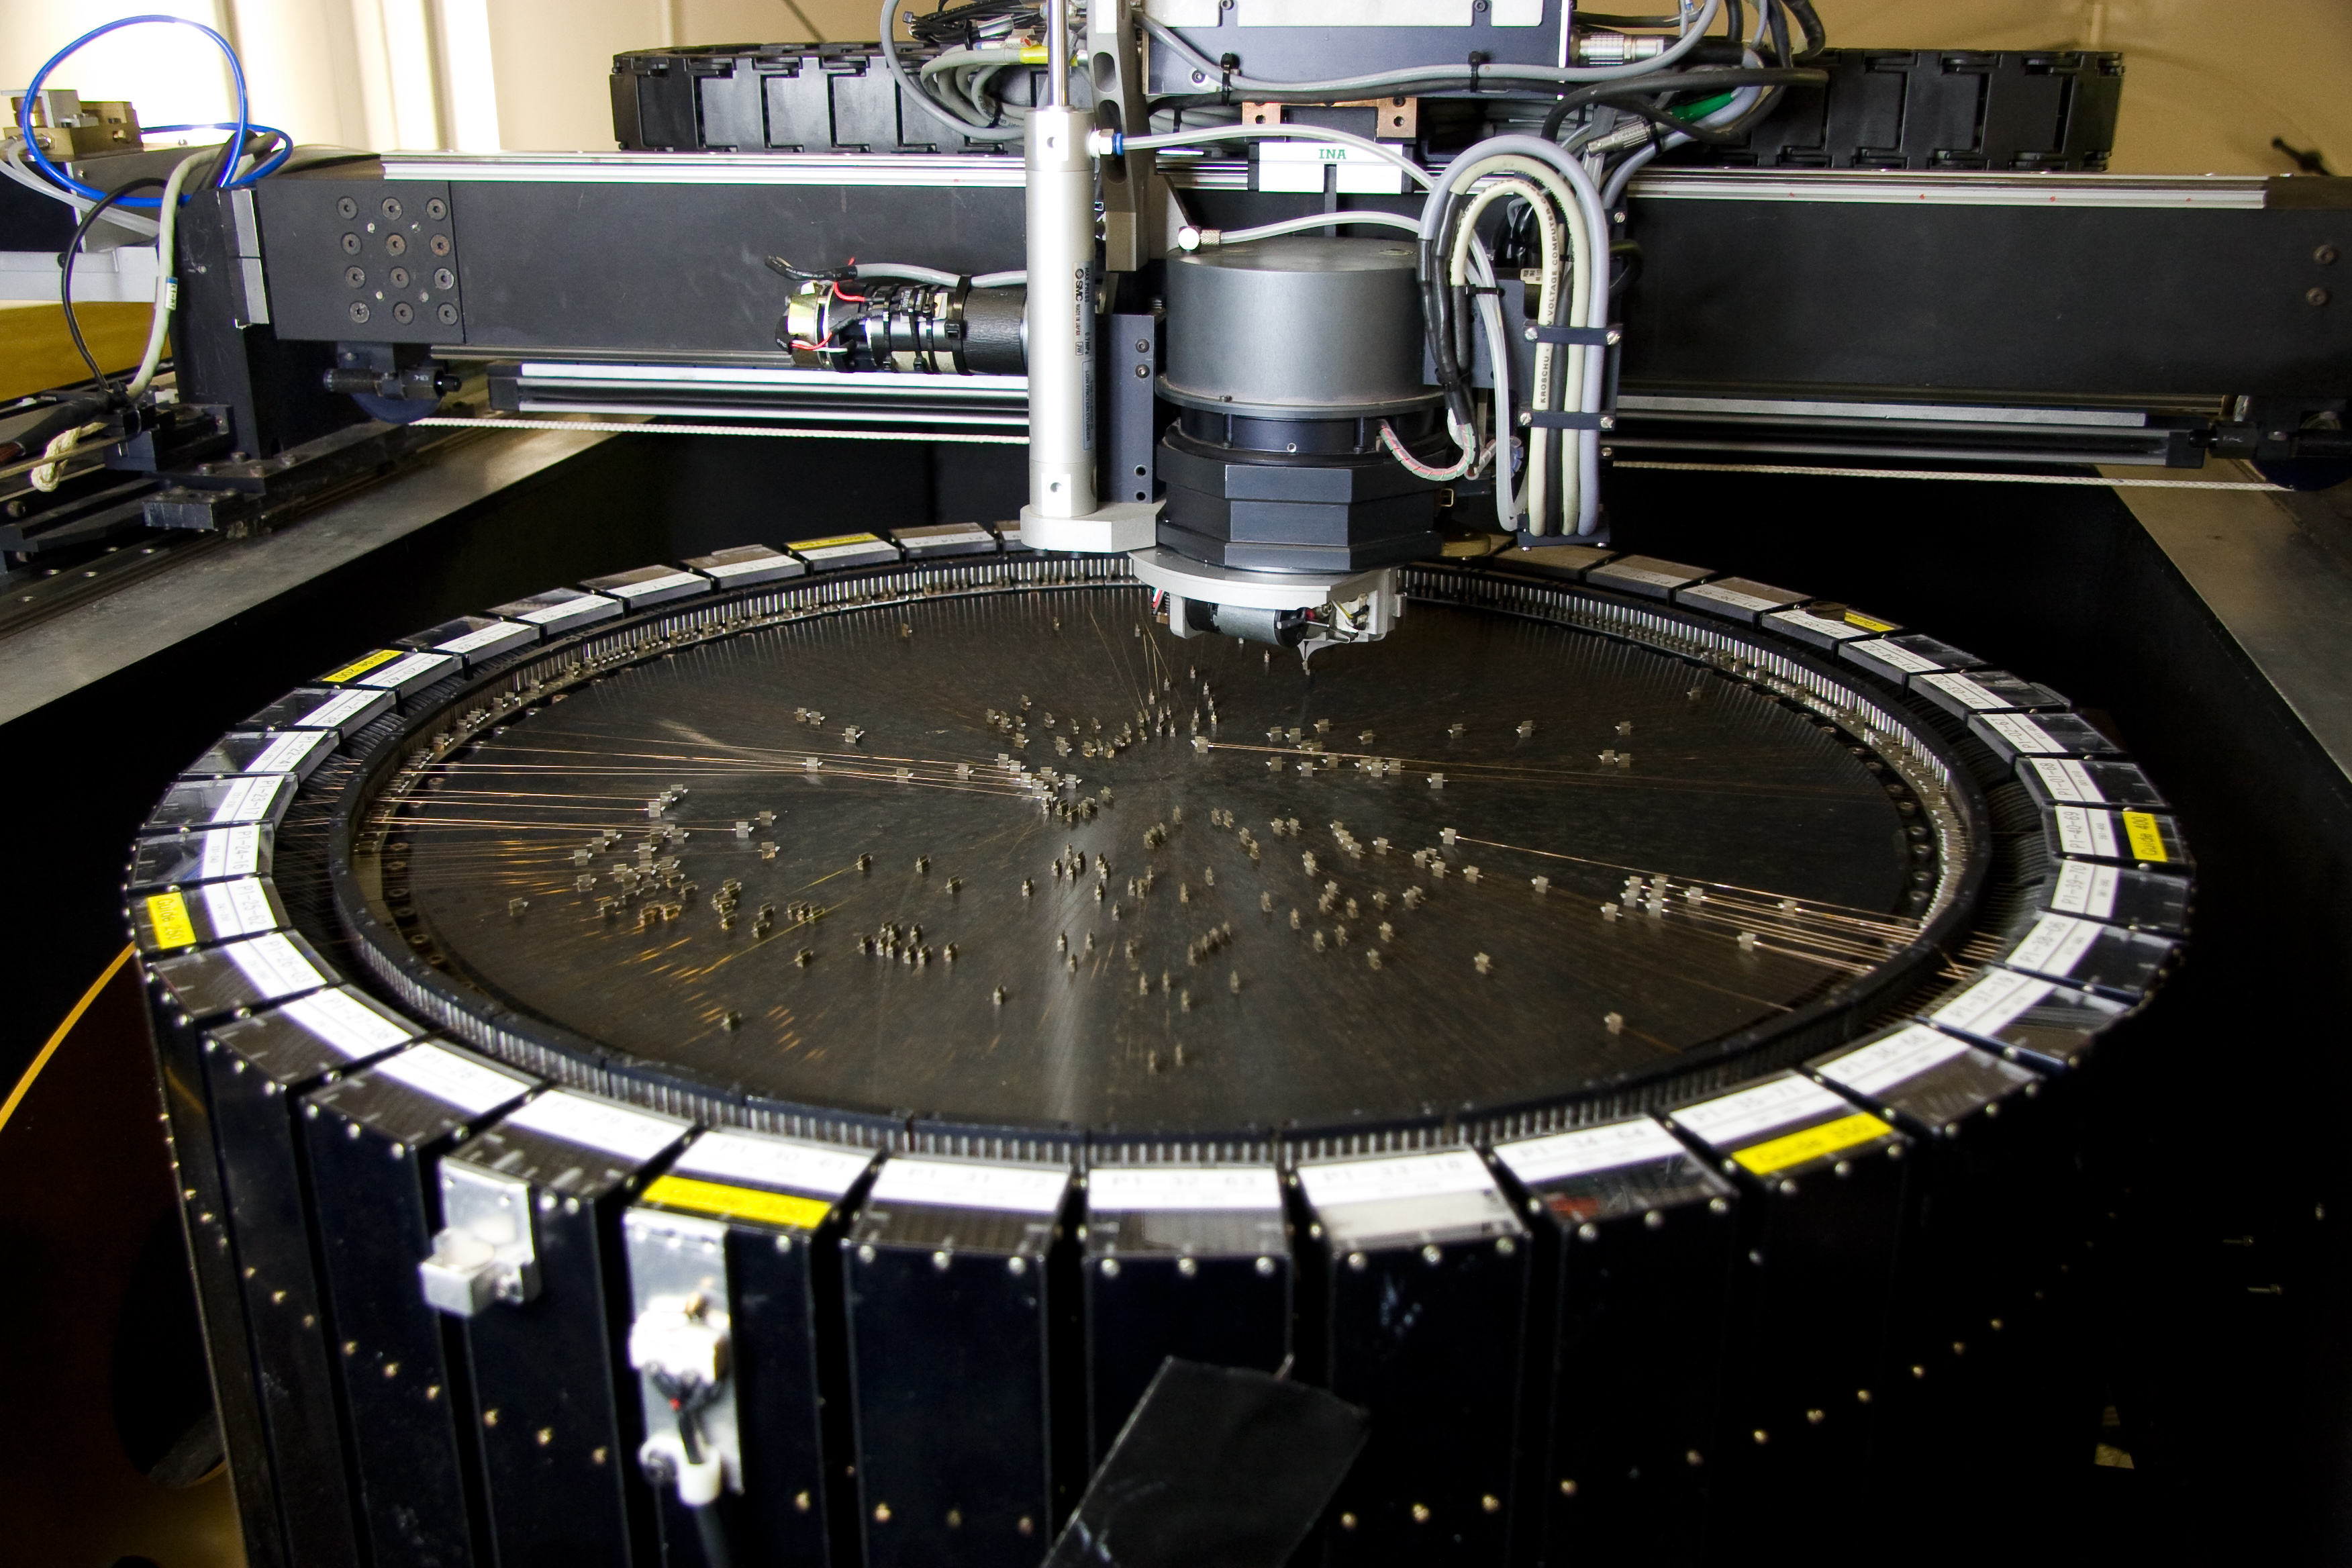
\includegraphics[width=0.48\columnwidth]{2df.jpg}
	\includegraphics[width=0.48\columnwidth]{Optical-layout-of-the-HERMES-spectrograph.png}
	\caption{Crucial parts of the HERMES spectrograph are 2dF fiber positioner (left image) and four individual spectrograph arms.}
	\label{fig:hermes_2df}
\end{figure}

The GALAH survey was the main driver for the construction of the High Efficiency and Resolution Multi-Element Spectrograph (HERMES, \cite{2010SPIE.7735E..09B, 2015JATIS...1c5002S}), a multi-fibre spectrograph mounted on the $3.9$-metre Anglo-Australian Telescope (AAT) situated at the Siding Spring Observatory, Australia. The spectrograph has a resolving power of R $\sim 28,000$ (or R $\sim 45,000$ when slit mask is used) and covers four separately acquired wavelength ranges (4713 -- 4903~\AA, 5648 -- 5873~\AA, 6478 -- 6737~\AA, and 7585 -- 7887~\AA), together covering approximately 1000~\AA, including the H$\alpha$ and H$\beta$ lines. The ranges are frequently referred to as blue, green, red and near-infrared spectral arms (see left image of Figure \ref{fig:hermes_2df}). This configuration can simultaneously record spectra from up to 392 fibres distributed over a $2^\circ$ diameter field of the night sky, with an additional 8 fibres used for the telescope guiding. The fiber positioner has two identical plates that are used to precisely position fibers at designates stellar locations. During the exposure with the first plate, the robotic positioner is placing fibers on the second plate as shown in Figure \ref{fig:hermes_2df}. The complete fiber allocation process takes about half an hour per plate. The spectrograph can typically achieve a signal to noise ratio (SNR) $\sim100$ per resolution element at magnitude V=14 in the red arm during an 1-hour long exposure. To achieve as high SNR as possible and minimise atmospheric diffraction, all observations are ideally done when an observed field is passing through the meridian. With a fibers' finite field of view of 2\arcsec, we also want the object to be as high as possible on the sky. Observing at low altitudes could diffract different wavelengths over an angle that is larger than the fiber entrance point. Something that is not desigread as one of the spectrograph arms would receive less photons than others

\subsection{Acquired spectra and target selection}
The spectroscopic data used during the production of this thesis were taken from the pilot survey, the main GALAH survey \cite{2015MNRAS.449.2604D}, the K2-HERMES survey \cite{2018AJ....155...84W}, the TESS-HERMES survey \cite{2018MNRAS.473.2004S}, and specially dedicated the HEMRES open clusters (De Silva et al. in preparation) and the HERMES Orion star-forming region (Kos et al. in preparation) surveys. Together they form a dataset of $669,845$ successfully reduced stellar spectra, of which a small fraction belongs to repeated observations. All acquired spectra are homogeneously reduced to one-dimensional spectrum, normalised and shifted to the stellar reference frame (detailed description in \citet{2017MNRAS.464.1259K}). Combination of those surveys produces an increased number of spectra compared to the main GALAH survey. However, at the same time, this breaks the rule of a simple, unbiased selection function (Sharma et al. in preparation) that is desired for population studies and easier comparison with synthetic galactic models.

The original selection function of the main GALAH survey is separated into two magnitude limited field selections - bright (10<V<12) and regular (12<V<14) fields whose target selection is colour independent. Used V magnitude is inferred from magnitudes measured by the Two Micron All-Sky Survey (2MASS) \cite{2006AJ....131.1163S} whose photometric bands are shifted into the infra-red spectral region. Because of that, some, especially peculiar and variable stars, might have an erroneous estimation of V magnitude leading to underexposure or excessive spectral crosstalk. Because of expected crowding problems (projected diameter of used optical fibre on the sky is equal to $2$\arcsec) observed stars are located at higher Galactic latitudes ($|b|$~>~$10^\circ$) where the density of stars is lower. Additional surveys sometimes break those rules by selecting fainter/dimmer stars, going closer to the Galactic plane, employ colour cuts, or favour interesting preselected stars such as K2 \cite{2014PASP..126..398H} targets, TESS \cite{2015JATIS...1a4003R} targets and cluster members. Therefore some care is needed when trying to infer global stellar or galactic properties based on such inhomogeneous selection criteria.

\subsection{Spectral reduction and parameters determination}
The first step after recording spectra in the form of a 2D image is their extraction to multiple 1D spectra. The procedure, extensively documented by \citet{2017MNRAS.464.1259K}, consist of the following steps: raw image cosmetic corrections, spectral tracing, optical aberrations correction, scattered light and apertures cross-talk removal, wavelength calibration, sky subtraction, and telluric absorption removal. After reduction, spectra are normalised and shifted into their rest-frame by cross-correlating them with a set of 15 AMBRE model spectra \cite{2012A&A...544A.126D}. This procedure produces initial velocities that are usable for parameter determination, but not accurate enough for possible inter-cluster analysis. The more precise methodology uses the GALAH observations itself to compute a much denser set of reference spectra for cross-correlation. Its details are described by \citet{2018arXiv180406344Z}. In the last step, the methodology also accounts for gravitational redshift and convective blueshift to determine actual stellar radial velocity. 

Stellar atmospheric parameters and individual elemental abundances are in a uniform way derived from all normalised spectra. The applied parameter analysis pipeline slowly evolved and improved during the GALAH survey. The three most important milestones in an ongoing process are:

\begin{itemize}
	\item The initial stellar parameters (\Teff, \Logg, and \Feh), accompanying the first GALAH data release (\textbf{GALAH DR1}), were derived as a global fit (all arms at the same time) of the observed spectra to a grid of $16,783$ AMBRE spectra \cite{2012A&A...544A.126D}, which were convolved down to the average resolution of individual HERMES CCD. The aim of this procedure was to provide indicative stellar parameters, which could be used as a first initial guess to help speed up more complex stellar parameters and abundance pipelines.
	
	\item The parameters (with extension to \vsin, \vmic, and \aks) and up to 23 elemental abundances, released as part of the \textbf{GALAH DR2} \cite{buder2018}, were produced using the multi-step data-driven approach. The complete analysis depended on a set of $10,605$ spectra that were selected in such way to span a large portion of the parameter space and did not contain any peculiar star, especially binary and emission line spectra. Selected spectra were analysed using a physics-driven spectrum synthesis code Spectroscopy Made Easy (\SM, \cite{1996A&AS..118..595V, 2017A&A...597A..16P}) that performs spectrum synthesis for 1D stellar atmosphere models. In the case of DR2, it consists of MARCS theoretical 1D hydrostatic models \cite{2008A&A...486..951G} under the assumption of local thermodynamic equilibrium (LTE) for the majority of elements. The procure is computationally efficient but does not completely describe the physics inside stars. Therefore several vital elements (Li, O, Na, Mg, Al, Si, and Fe) were analysed using more realistic non-LTE line formation. A common approach to compute non-LTE abundances is to use the same pipeline as for LTE but internally account for the non-LTE departure coefficients that were in advanced computed using complex non-LTE computations that account for realistic atom collisions. Such departure coefficients are usually computed for a limited grid of stellar parameters and afterwards interpolated in between when need \cite{2020A&A...637A..80O, 2019A&A...630A.104A, 2020amarsigalah}.
	
	To propagate the parameter and abundance results of the training set to the whole survey, \TC\ \cite{2015ApJ...808...16N} generative data-driven approach was used. It adopts a simple quadratic model which uses stellar parameters to describe the observed flux of a given spectrum. Independent model is built for every spectrum wavelength pixels. To train \TC\ model, all spectra in the training set were interpolated to a common wavelength grid. After the training is performed, the model was inverted to produce parameters and abundances for every observed spectrum by fitting it to the internal generative spectrum produced by \TC. Further details of the described process are given in \citet{buder2018}.
	
	\item Not relying on the GALAH spectral information alone, but including \G\ parallax, colour, and absolute magnitude, additional constraints and priors can be used to infer spectroscopic stellar parameters. That additional information can be used to confine information about \Logg\ and stellar age. Adaption of \SM\ software, thoroughly described in \citet{buder2020}, was used to accommodate additional \G\ information in order to produce the latest \textbf{GALAH DR3} data set. Unlike in DR2, no data-driven methodology was used to produce stellar parameters and abundances as \SM\ was run for every individual normalised spectrum. Reference spectra were generated using MARCS 1D stellar models. For eleven abundances (out of 30 measured) non-LTE corrections were performed. The published catalogue contains several additional Value-Added-Catalogues defining stellar ages and their galactic dynamics. To compute stellar masses and ages, the best matching PARSEC+COLIBRI isochrone was used.
	
	With the addition of so many auxiliary information with their own uncertainties, that are sometimes not even known or unable to be estimated, the question arises if they also impact the quality of the published results. As the precise parameters and abundances are the driving focus of the ongoing survey, we tried to estimate the possible trend and offsets by analysing open clusters in Chapter \ref{chap:clusters}.
	
\end{itemize}

\section{Asiago spectroscopic observations}
\label{sec:asiago_data}
Vastly different from the previous two massive all-sky surveys, telescopes at the Asiago site are mainly used for dedicated observations or monitoring of previously selected targets whose observational and astrophysical potential was identified from all-sky surveys. During our stay at the Asiago Observatory, that usually lasted for four consecutive bright nights (close to full Moon) every month, we used the $1.82$~m Copernico telescope located on top of the nearby hill Mount Ekar (Asiago, Italy - the altitude of $1,366$~m).

Our observations were performed by the Echelle spectrograph that is during near-full Moon days mounted on the telescope. At that time, the quality and deepness of photometric observations are heavily reduced and therefore not performed. Design of the Echelle instrument and its slit length enables the observer to observe only one star a time. Obtained spectra have a resolving power of R$\sim20,000$ and a wide span of wavelengths between $3600$ and $7400$ \AA. They are divided into 30 interference orders which partially overlap with succeeding and preceding order, providing an undisturbed coverage of observed wavelengths. Acquired spectra were recorded by the Andor DW436-BV CCD camera. The camera uses a back-illuminated CCD detector with a size of $2048 \times 2048$ pixels. This setup enables us to capture spectra of stars with magnitudes V~<~$10$ at high SNR with reasonable exposure time (less than 1 hour per spectrum). Because of the mechanical limitation, observed stars must be positioned at least $15^\circ$ above the local horizon. At those low altitudes, only the brightest stars are reasonable to be observed because of strong atmospheric attenuation and diffraction differences between red and blue wavelengths. The latter effect can be reduced by rotating the slit of the spectrograph into the paralactic angle.

Combining the location of the observatory and above observational limitations with the fact that our exciting stars were in advance selected from the GALAH survey, highly reduces the number of potentially observable objects. To reduce the atmospheric effects, we observed only stars which rose at least $30^\circ$ above the local horizon. This minimum altitude limitation is equal to omitting observable candidates as to having $\delta$~<~$-15^\circ$. As described in more detail below (see Chapters \ref{chap:peculiars_chem} and \ref{chap:twins}), we used additional Asiago observations to inspect spectroscopic features not accessible by the GALAH spectra and to prolong radial velocity time series of possible multiple stars who could show signs of radial velocity changes not detectable by a single epoch GALAH spectrum.

Additionally, to our program observations, we also contributed spectroscopic observations that resulted in published astronomer's telegrams \cite{2019ATel13340....1M} and scientific papers \cite{2019MNRAS.488.5536M}.

\chapter{Chemo-dynamic tracing of open cluster stars}
One of the main goals of the \Gh\ survey is to explore possibilities of chemical tagging for random field and known open cluster stars. A task that sounds easy in theory, but its working applications are far from ready for large spectroscopic surveys. The road to getting precise stellar chemical abundances leads around many different obstacles, which all have an impact on the final determined abundance values whose precision and accuracy dictates the possibility and success of implementing chemical tagging.

In this chapter, we present our exploration of abundances for a few open clusters that were observed during multiple different surveys run by the HERMES spectrograph. In Section \ref{sec:intro_tag}, we briefly describe the history of open cluster membership, the evolution of clusters, and means to discover these ongoing processes using stellar abundance information only. Of multiple sparsely observed open cluster in the GALAH, we focus only on a small subset of them that have the highest number of members (see Section \ref{sec:galah_clusters} for the complete list). Section \ref{sec:membership_v2} describes the selection of clusters and integration of orbits for stars inside and around the clusters. Chemical signature of field and cluster stars is analysed in Section \ref{sec:chem_ej_tag} and the results summarised and discussed at the end of this chapter.

\section{Introduction}
\label{sec:intro_tag}
The latest second release of \G\ data \citep[DR2,][]{2018arXiv180409365G} revolutionized numerous fields of astronomy, including research of galactic open clusters. Its combined information of stellar distance, kinematics, and photometric measurements enables us to go beyond simple methodologies, such as star density counts, to unravel even the faintest and sparsest components of open clusters. So far, many works have been published trying to refine parameters, and membership information of long known open clusters \citep{2017A&A...601A..19G, 2018A&A...618A..93C, 2019A&A...627A..35C} and find new, less numerous or fainter clusters \citep{2019ApJS..245...32L, 2019JKAS...52..145S, 2019A&A...624A.126C, 2020arXiv200107122C}. Such thorough and the improved investigation uncovered that many of the clusters listed in modern catalogues, initially discovered as apparent stellar overdensities, are no more than chance alignments of stars and not true physical clusters \citep{1998A&A...340..402B, 2000A&A...357..145C, 2016AJ....152....7H, 2018MNRAS.480.5242K, 2020A&A...633A..99C}.

Born from the same molecular cloud, open clusters are ideal test structures for different astrophysical principles. Being influenced by external and internal processes, such as tidal stripping and close stellar interactions, their lifetime is limited from about 100 Myr to a few Gyr for the densest structures \citep{1998A&A...337..363P, 2013MNRAS.434.2509M}. This gives us a possibility of observing them at different evolutionary stages \citep{2006BASI...34..153C, 2007A&A...468..139P} before they blend \citep{2001A&A...366..827B} into field stellar population. The most prominent transitional features we can observe are compact cluster tidal tails \citep{2019AA...627A...4R, 2019AJ....157..115Y, 2019AA...621L...3M, 2019arXiv191206657Z} and lose extended halos of evaporated stars. They are observed as a slowly decreasing over-density \citep{2002A&A...385..471C, 2004A&A...427..485B, 2019AA...627A.119C} of stars far from a denser cluster core. Due to close gravitational interactions among members, they can be ejected out of a cluster at high velocities \citep{2009MNRAS.396..570G, 2010MNRAS.402..105G, 2017MNRAS.470.3049R}. Such cluster members can on the sky be found even several degrees away from their main cluster body \citep{2007MNRAS.376L..29G, 2018MNRAS.473.4612K, 2019ApJ...884....6M}.

Majority of the described works relied on a complete 6D positional and kinematics information to discover clusters and their sub-structures. Advances in observational techniques and data analysis enables us to go beyond kinematics information and include a multidimensional chemical signature of stars -- a procedure known as chemical tagging \citep{2002ARA&A..40..487F, 2010ApJ...721..582B}. So far blind chemical tagging (without kinematics) of cluster and field stars has not yet been demonstrated with great success unless the observed structure has obviously different chemical composition \citep{2016ApJ...833..262H}. A trait that it is not common to open clusters formed at about the same time \citep{2019A&A...629A..34G}, but to galactic components formed at vastly different epochs \citep{2018A&A...619A.125A}.

The latest research showed that many, even unexpected, observational and data reduction issues still have to be thoroughly investigated and resolved, especially if data from different surveys are to be combined \citep{2019ARA&A..57..571J}. Studies suggest that open clusters might not be as homogeneous as thought before \citep{2016ApJ...817...49B, 2018MNRAS.473.4612K} as abundances trends show traits of dependency with stellar evolution \citep{2015A&A...577A..47B, 2017ApJ...840...99D, 2018MNRAS.478..425B}. On top of that, main concerns of chemical tagging are spectra analysis induced abundance trends \citep{2016ApJ...817...49B, 2019arXiv191208539C, 2020arXiv200103179B} that depend on determining underlying stellar physical parameters (i.e. \Teff\ and \vsin) which usually are not changed or fitted during abundance determination procedure. Observed trends might also be results of inadequate stellar models or actual stellar processes. To cope with this complexity and uncertainties, complex Bayesian models are being developed \citep{2016ApJ...817...49B, 2019ApJ...887...73C} in order to uncover and cluster abundance patterns. With this in mind, many work and validation still have to be done until large surveys are fully ready for blind chemical tagging experiments. 

\section{Additional data specifics}
\label{sec:data_clusters}

\subsection{The GALAH and cluster stars}
\label{sec:galah_clusters}
Among the dedicated HERMES cluster observations and other surveys, such as the \Gh, we detected members of know open clusters, whose stellar membership was taken from results published by \citet{2018A&A...618A..93C}. As some of the clusters were not targeted intentionally by the surveys or only their cores, the number of observed member and surrounding field stars of interest can vary substantially. The clusters analysed in this paper, having the most significant number of spectroscopic observations are Berkeley 32, NGC 2516, NGC 2112, NGC 6253, Blanco 1, Ruprecht 147, NGC 2632, NGC 2682,  Melotte 22, and Collinder 261. To supplement their selection, we added members of Melotte 25 cluster whose membership selection was performed by us as it was missing in the mentioned published paper \cite{2018A&A...618A..93C}. \rb{Naceloma sem imel en cel Section tega, vendar ne pride sedaj v postev ce se uporabi vecinoma objavljena clanstva}

\subsection{Gaia}
\label{sec:gaia_clusters}
For a complete 6D positional and kinematics stellar information, we augmented the \Gh\ data with proper motion, parallax and radial velocity from the \Gs\ data-set. As all of the investigated open cluster stars are located close to the Sun, their distances can be inferred by inversion of a parallax value as $1 / \varpi$. The current release of the \G\ data contains magnitude limited range of recovered radial velocities, that are, whenever possible, supplemented or substituted with the \Gh\ measurements of higher accuracy \cite{2018arXiv180406344Z}. Supplemented are mostly stars fainter than currently adopted \G\ RVS \cite{2018A&A...616A...5C} analysis threshold as the GALAH targets are much fainter stars than the RVS limit. The synergy, therefore, increases the set of useful stars in our case.

\section{Cluster membership}
\label{sec:membership_v2}
The first step in our analysis was the acquisition of data relevant for each cluster identified among the \Gh\ observations. Identification of observed clusters was made by matching observed stars with known cluster members published by \citet{2018A&A...618A..93C}. As some of the clusters had a low number of stars or were proved to be chance alignments of stars \citep{2018MNRAS.480.5242K}, they were not considered in the analysis. Sky coordinates and distances of selected open cluster members (see Section \ref{sec:galah_clusters} for the list of considered clusters) were taken from \citet{2018A&A...618A..93C} and served us as anchors around which we queried the \Gs\ data. A cone query with a radius of $6^\circ$ and distance limit of $\pm900$~pc around a cluster centre was performed to download a subset of the whole dataset. This downloaded subset included stars with an incomplete set of \G\ parameters. To complement and improve quality of radial velocity measurements, all available the \Gh\ velocity estimates in a subset were used to override or supplement \G\ measurements. In the case of multiple the \Gh\ observations, a median velocity per star was used.

The initial open cluster memberships were taken from \citet{2018A&A...618A..93C}, but needed some refinement before it was suitable for us. To select as many possible cluster members, the employed membership algorithm did not relay on magnitude limited radial velocity information to assign cluster membership. To make cluster volume compacter and retain only the most probable members, we discarded all member stars whose radial velocity deviated for more than $5$~\kms\ from the cluster median value of all retrieved members.

\subsection{Stellar tracing}
\label{sec:orbit_tracing}
After the selection of open cluster members, we proceeded with the analysis of stellar movements inside and outside the cluster. In order to get the most reliable motion information, only stars with a complete 6D kinematic information (proper motion + radial velocity + sky coordinate + parallax) were considered. No additional \G\ quality flagging was used to remove stars with potentially bad parameter estimates as we would, in the following steps, like to show that they could be discovered and eliminated based solely on their chemical composition.

By knowing members of the observed clusters and their current position and complete motion vectors, we can trace the path of a volume constrained by the cluster stars backwards or forwards in time. This integration procedure was performed by individual integration of cluster stars in axisymmetric gravitational potential \citep[\textit{MWPotential2014} potential,][]{2015ApJS..216...29B} using \GP\ software library \citep[version 1.5.0.,][]{2015ApJS..216...29B}. Being interested in the past ejected members of a cluster, we integrated orbits of cluster stars for $120$~Myr (comparable to ages of the youngest open clusters in our set) into their past and saved their location after every step of $20$~kyr. As the integration process relies only on the present uncertain measurements of their velocities and distance, longer integration is not precise or reliable. This is observed by the fact that cluster volume gets larger during backwards integration instead of getting smaller. At every integration step, the cluster volume was described by a minimum convex hull defined by its outer-most members. Such a geometrical shape presents the smallest bounding volume with partially flat boundaries which encompasses all considered members.

The next step of our analysis consisted of finding spatially nearby stars that could be traced back to having origin in a considered open cluster. To filter out field stars that travel into completely different direction than a cluster, we discarded all stars whose galactic velocity vector difference towards present cluster velocity vector was >$50$~\kms. \rb{a je to sploh smiselno? prihranek racunskega casa je nekje polovica} Orbits of remaining set of stars (usually more than half of queried stars) were integrated using the same configuration as cluster stars. A this point, we could investigate which orbit of field stars crosses clusters' volume at any given integration step.

To get a more descriptive crossing probability, we created $250$ incarnations of every field star. Initial kinematic properties of each incarnation were drawn from Gaussian distributions of parallax, radial velocity, and proper motion defined by their reported value and uncertainty. After analysing all $250$ orbits of each star, we described its cluster crossing probability by the longest stay inside the cluster volume and percentage of crossing events. For a crossing to be counted as confirmed, a star had to be located inside the cluster volume for at least $0.4$~Myr, time that is equivalent to $20$ integration steps. The final selection of probable ejected stars consist of stars, whose integration procedure revealed that they were crossing a cluster volume in at least $68$\% of incarnations and their longest stay there was at least $1$~Myr. Remaining volume crossing stars, that did not met the criteria, were not considered as field stars, but were discarded from further analysis as they might pollute chemical signature of a field population. Summary of investigated and discovered stars for every cluster is given in Table \ref{tab:cluster_stats}.

\begin{table}
	\centering
	\caption{Cluster statistics. Only stars with a complete 6D positional and kinematic information were considered for this statistics and orbit integration analysis. Number in columns successively present number of all star with complete information, number of analysed stars that meet initial criteria of having velocity similar to a cluster, number of stars that do not cross cluster volume during integration, number of probable ejected stars, and number of cluster members that defined volume of a cluster.}
	\begin{tabular}{l | c | c | c | c | c }
		\hline
		Cluster & All & Analysed & Field & Ejected & Members \\
		\hline
		Berkeley 32  & 11322 & 2659 & 2047 & 125 & 23 \\ 
		Blanco 1     & 5043 & 2734 & 2687 & 15 & 81 \\
		IC 4665      & 15022 & 10155 & 9823 & 26 & 34 \\
		Mamajek 4    & 21776 & 11623 & 10513 & 85 & 48 \\
		Melotte 22   & 9097 & 6335 & 5944 & 105 & 239 \\
		Melotte 25   & 0 & 0 & 0 & 0 & 0 \\
		NGC 1817     & 12826 & 4489 & 4060 & 74 & 54 \\
		NGC 1901     & 12666 & 7323 & 7204 & 19 & 30 \\
		NGC 2112     & 13866 & 6665 & 6323 & 38 & 49 \\
		NGC 2204     & 4314 & 1777 & 1170 & 180 & 59 \\
		NGC 2516     & 17383 & 11906 & 11030 & 315 & 182 \\
		NGC 2548     & 14371 & 9212 & 8842 & 60 & 34 \\
		NGC 2632     & 9951 & 5290 & 4991 & 170 & 222 \\
		NGC 2682     & 10947 & 5244 & 4776 & 226 & 287 \\
		NGC 6253     & 62975 & 30114 & 17267 & 1362 & 64 \\
		Ruprecht 147 & 17749 & 5062 & 4850 & 23 & 103 \\
		\hline
	\end{tabular}
	\label{tab:cluster_stats}
\end{table}


\section{Chemical signature of clusters}
\label{sec:chem_cluster}
After defining potential members of different cluster components (field, ejected, and members), we can look into abundance signatures of an individual component. Of all 29 possible The \Gh\ chemical abundances, we initially excluded only Li because of its intrinsic variability that depends on stellar evolutionary stage. Scatters plots of all considered abundances and \Feh\ as a function of stellar effective \Teff\ for different clusters are shown in Figures \ref{fig:ct_cluster1}, \ref{fig:ct_cluster2}, \ref{fig:ct_cluster3}, and \ref{fig:ct_cluster4}. Not all plots for the same cluster have equal number of points as reporting of abundance values depends on estimation of their reliable detectability that is based on equivalent widths of element absorption lines \citep[thoroughly described in][]{buder2020}. The plots show only stars with unflagged \citep[\texttt{flag\_sp} = 0, described in][]{buder2020} stellar parameters. 

\begin{table}
	\centering
	\caption{Number of acquired the \Gh\ spectra among different cluster components that were considered during the chemical comparison. No parameter or abundance flagging was yet used at this point. Stars represented by this statistics are a subset of stars given in Table \ref{tab:cluster_stats}. Because of repeated observations, some clusters (especially NGC 2682 that was used as a calibration filed) can have a higher number of spectra than member stars.}
	\begin{tabular}{l | c | c | c }
		\hline
		Cluster & Field & Ejected & Members \\
		\hline
		Berkeley 32  & 0 & 0 & 0 \\ 
		Blanco 1     & 0 & 0 & 0 \\
		IC 4665      & 0 & 0 & 0 \\
		Mamajek 4    & 0 & 0 & 0 \\
		Melotte 22   & 0 & 0 & 0 \\
		Melotte 25   & 0 & 0 & 0 \\
		NGC 1817     & 0 & 0 & 0 \\
		NGC 1901     & 0 & 0 & 0 \\
		NGC 2112     & 0 & 0 & 0 \\
		NGC 2204     & 0 & 0 & 0 \\
		NGC 2516     & 0 & 0 & 0 \\
		NGC 2548     & 0 & 0 & 0 \\
		NGC 2632     & 0 & 0 & 0 \\
		NGC 2682     & 0 & 0 & 0 \\
		NGC 6253     & 0 & 0 & 0 \\
		Ruprecht 147 & 0 & 0 & 0 \\
		\hline
	\end{tabular}
	\label{tab:cluster_stats_abund}
\end{table}

\subsection{Abundance trends}
\label{sec:abund_trends}
%Ker vidimo in tudi drugi modeli kar mocne trende zastopanosti v odvisnosti od fizikalnih parametrov zvezd, je treba te nekako spraviti na isto raven. Najlazje diferencialno - naredimo fit na kopico in gledamo koliko ostali odstopajo od tega
The first thing we noticed on the shown abundance scatter plots is their strong dependence with physical parameters, especially \Teff. As this is not the first or unique observation of those trends \citep{2010A&A...523A..71G, 2013ApJ...775...58B, 2016MNRAS.457.3934L, 2018A&A...619A.176B, 2019arXiv191208539C}, they are most likely partial products of insufficient/inaccurate stellar models or actual abundance patterns, and not induced solemnly by the employed \SME\ spectrum analysis pipeline \citep[][]{buder2020}.

If we presume that observed trends are artificially induced and clusters should have homogeneous chemical composition that is independent of stellar type, a differential analysis can be used. Such analysis considers only comparisons among stars with a similar set of stellar parameters. To describe observed trends, we independently fitted a 3$^{rd}$ degree polynomial function using $2.5\sigma$ clipping algorithm in 2 steps to every abundance versus \Teff\ diagram. By subtracting fitted trends, we estimated degree of intra cluster scatter for every element. Because of limitations of measuring certain abundances, the fit was not performed if number of points was lower or equal to a used polynomial degree $+1$.

\rb{Nekam lahko morda pride se primerjava razprsenosti zastopanosti med posameznimi elementi in posameznimi kopicami.}

\subsection{Chemical membership}
\label{sec:chem_ej_tag}
%Pogledamo trende in fite, ter koliko moznih izvzenih zvezd se poraja in sklada s temi kemicnimi trendi. Morda nek threshold koliko je dobrih oziroma skladnih s samo kopico, saj ima tudi ta le kar nekaj razpona v izmerjenih/izracunanih vrednostih parametrov.
Having an analytical description of an individual abundance behavior for every cluster, we can estimate how many and how accurately do the identified ejected stars match with cluster abundance patterns and trends. The most straightforward way to perform this is to count how often does abundance value of an investigated star falls inside a $1\sigma$ (or $2\sigma$ for a more relaxed selection) region around an abundance trend. Before performing such counting, we additionally omitted abundance trends of the following chemical elements: V, Rb, Sr, Y, Zr, Mo, Ru, La, and Sm. Their low number of successful measurements per cluster and uncertain trends were not beneficial to the whole chemical tagging experiment and influenced only a small fraction of stars. \rb{nacelona tega sploh ne zelimo delat, samo eni so vizualno res cudni} A star was counted as chemically similar if it matched to a cluster in at least $68$\% of considered abundances.

\subsection{Tagging remaining field stars}
\label{sec:chem_fi_tag}
%Kaj se zgodi ce iste kemicne informacije in thresholde uporabimo se za ostale analizirane zvezde v bljizini. Dobimo sploh kaj zvezd ven iz tega in kaksen bi bil v tem primeru njihov kinematicni vektor.
The same principle can also be applied to remaining nearby field stars. As clearly evident from Figures \ref{fig:ct_cluster1}, \ref{fig:ct_cluster2}, \ref{fig:ct_cluster3}, and \ref{fig:ct_cluster4}, the cluster abundances are mostly similar to field stars and lie close to their densest regions in a scatter plot. Therefore, we were interested into the probability of a field star being chemically similar to a nearby cluster. In contrast, some of the investigated clusters, especially Blanco 1, showed evident signs of being chemically separable from neighboring populations in few abundances that are commonly used as chemical tracers of galactic evolution and stellar age \citep{2003A&A...410..527B, 2018MNRAS.474.2580S, 2020MNRAS.491.2043L}.

For a field chemical tagging procedure, we used the same selection principle as previously described in Section \ref{sec:chem_ej_tag}. The results of both tagging experiments are presented in Table \ref{tab:cluster_stats_abundtag}.

\begin{table}
	\centering
	\caption{Number and percentage of all considered and chemically similar (tagged) stars in the spatial neighborhood around analysed open clusters. Percentages indicate number of stars in different components that are similar to cluster abundance pattern and scatter. Selection algorithm is detailed in Section \ref{sec:chem_ej_tag}. Only spectra with unflagged stellar parameters were used to produce shown statistics.}
	\begin{tabular}{l | c | c | c | c }
		\hline
		Cluster & \multicolumn{2}{c}{Ejected}  & \multicolumn{2}{c}{Field} \\
		 & All & Tagged & All & Tagged \\
		\hline
		Berkeley 32  & 2 & 0 (0.0\%) & 39 & 0 (0.0\%) \\ 
		Blanco 1     & 4 & 2 (50.0\%) & 99 & 3 (3.0\%) \\
		IC 4665      & 4 & 0 (0.0\%) & 905 & 0 (0.0\%) \\
		Mamajek 4    & 25 & 7 (28\%) & 2273 & 136 (6.0\%) \\
		Melotte 22   & 10 & 1 (10\%) & 708 & 76 (10.7\%) \\
		Melotte 25   & 12 & 4 (33.3\%) & 639 & 4 (10.6\%) \\
		NGC 1817     & 6 & 0 (0.0\%) & 427 & 6 (1.4\%) \\
		NGC 1901     & 19 & 4 (21.1\%) & 5510 & 1034 (18.8\%) \\
		NGC 2112     & 4 & 0 (0.0\%) & 268 & 8 (3.0\%) \\
		NGC 2204     & 19 & 3 (16.7\%) & 113 & 14 (12.4\%) \\
		NGC 2516     & 70 & 4 (5.7\%) & 3285 & 72 (2.2\%) \\
		NGC 2548     & 5 & 0 (0.0\%) & 603 & 6 (1.0\%) \\
		NGC 2632     & 56 & 7 (12.5\%) & 1523 & 74 (4.9\%) \\
		NGC 2682     & 85 & 32 (37.6\%) & 1133 & 253 (22.3\%) \\
		NGC 6253     & 27 & 3 (11.1\%) & 648 & 28 (4.3\%) \\
		Ruprecht 147 & 9 & 0 (0.0\%) & 559 & 23 (4.1\%) \\
		\hline
	\end{tabular}
	\label{tab:cluster_stats_abundtag}
\end{table}

\section{Comparison with known remains}
\label{sec:tails_chem}
%Izvedli bi krajso primerjavo kako v luci nasih dognanj vidimo plimske repe kopic, ki so jih zaznali drugi.
In the previous section we analysed stars whose orbits indicate that they could be ejected from open clusters sometime in their past. Depending on a mass of involved stars and their proximity during the slingshot mechanism, stars could be thrown out of the cluster into inter-stellar space at various velocities and directions. 

A less energetic and more gradual mechanism that also influences lifetime of an open cluster is tidal stripping of stars \citep{2006A&A...455L..17L}. It happens during clusters' journey trough more heavily populated regions such as spiral arms. In this section we compare kinematics and chemical composition of known tidal structures \citep[discovered in \Gs\ data by ][]{2019AA...627A...4R, 2019AA...627A.119C, 2019AA...621L...3M, 2019arXiv191206657Z} of a few \Gh\ clusters with other previously analysed structures.

\subsection{Kinematics comparison}
Ali je njihova kinematika sploh taksna da integracija njihovi orbit kaze nazaj proti volumnu kopice ali pac ne. Ce ne, imamo morda neko potrditev da res isceno izvrzene in ne strukture nekih pocasnih gravitacijskih vplivov??

First we compared their measured kinematics and position to determine if it would be possible to select the same subset only on those properties, without prior knowledge that they might once be a part of a nearby dissolving open cluster. \rb{nisem se kaj veliko tega gledal}

\subsection{Tidal tails chemistry}
Kaj pa pravi njihova kemicna sestava na povezavo s kopico in ali imajo enake galah podpise? Ce ne, se je treba spomnit kaj pametnega zakaj bi lahko temu bilo tako. Ne deluje teorija, analiza nasih podatkov ali pa pac niso bili formirani ob istem casu.

Among randomly acquired The \Gh\ spectra, we observed some stars that where identified to belong to kinematically discovered tidal structures around open clusters.

For a tidal tail chemical tagging procedure, we used the same selection principle as previously described in Section \ref{sec:chem_ej_tag}. The result of the tagging experiment is presented in Table \ref{tab:cluster_stats_tails}.

\begin{table*}
	\centering
	\caption{Opis te tabele. Tabela se v delu.}
	\begin{tabular}{l | c | c | c | c | c | r }
		\hline
		Cluster & Stars in & Without used & Common with & \Gh\ unflagged & Chemically & Tail membership\\
		 & reference & cluster members & ejected & parameters (\% in & tagged & reference\\
		 &  &  & (\% of ejected) & common with ejected) & (\% of valid) & \\
		\hline
		Blanco 1     & 644 & 276 & 4 (27\%) & 2 (100\%) & 0 (0\%) & \citet{2019arXiv191206657Z} \\
		NGC 2632  & 1393 & 738 & 37 (22\%) & 22 (68\%) & 0 (0\%) & \citet{2019AA...627A...4R} \\
		NGC 2682     & 952 & 241 & 20 (9\%) & 16 (81\%) & 0 (0\%) & \citet{2019AA...627A.119C} \\
		NGC 1817     & 0 & 0 & 0 (0\%) & 0 (0\%) & 0 (0\%) & \citet{a} \\
		Melotte 22   & 0 & 0 & 0 (0\%) & 0 (0\%) & 0 (0\%) & \citet{a} \\
		Melotte 25   & 0 & 0 & 0 (0\%) & 0 (0\%) & 0 (0\%) & \citet{2019AA...621L...3M} \\
		\hline
	\end{tabular}
	\label{tab:cluster_stats_tails}
\end{table*}

\section{Summary}
\label{sec:clusters_summary}

\section{Conclusions}
\label{sec:clusters_conclusions}

\begin{figure*}
	\centering
	\includegraphics[width=\textwidth]{p_teff_abundances_NGC_2682_orbits_DR3_flag0.png}
	\caption{NGC 2632 abundance scatter plots as a function of stellar effective temperature. The blue solid line represent the best fit on cluster population. The 1$\sigma$ and 2$\sigma$ abundance deviations from the fit are given by dashed lines of decreasing intensity. Coloured dots represent \ldots}
	\label{fig:ct_cluster1}
\end{figure*}

\begin{figure*}
	\centering
	\includegraphics[width=\textwidth]{p_teff_abundances_Blanco_1_orbits_DR3_flag0.png}
	\caption{Blanco 1.}
	\label{fig:ct_cluster2}
\end{figure*}

\begin{figure*}
	\centering
	\includegraphics[width=\textwidth]{p_teff_abundances_NGC_2632_orbits_DR3_flag0.png}
	\caption{NGC 2632.}
	\label{fig:ct_cluster3}
\end{figure*}

\begin{figure*}
	\centering
	\includegraphics[width=\textwidth]{p_teff_abundances_Ruprecht_147_orbits_DR3_flag0.png}
	\caption{Ruprecht 147.}
	\label{fig:ct_cluster4}
\end{figure*}

\chapter{Peculiar stars}
\section{Chemically enhanced stars}

\section{Multiple stars}

\section{Active stars}


\chapter{Conclusions}
The fast increase in observational data seen in the last decade with the introduction of new and improved astronomical observational facilities requires new approaches to the exploration of acquired data. The old mentally of exact and painstaking analysis of individual objects had to be changed in order to grasp the full potential of large observational sets. On the other hand, large amounts of data and complex observational scenarios also lead to more complicated data reduction and analysis pipelines. As it is impossible to look through all acquired data and consider all variables, many computer algorithms have over the years been developed to help with those tasks. Of them, the most trending and occasionally misused are numerous machine learning procedures of classification, clustering, and regression.

In this thesis, we used some of the available machine learning tools to explore large astronomical datasets, mainly collected as part of the \Gh\ and \G\ large sky surveys. The data of those surveys were, when needed, supplemented with results of other spectroscopic and photometric surveys. This merger gave us additional information by observing a broader wavelength range and an increase in temporal coverage of variabilities by combing similar data sets.

The body of this thesis focuses on exploring different types of stars. Usually, the stars are generally separated into two broad groups: normal and peculiar. The first term describes the majority of the stars that are happily living through the longest period of their lifetime. Being non-problematic, they are easily modelled and preferred for chemical analyses such as our exploration of open stellar clusters and their surrounding. During the analysis, we explored the possibility of chemical differentiation between chemical signatures of cluster members, possible past members and surrounding stars. Separation into given components for 11 open clusters was based on kinematic vectors defined by \G\ observations. The \Gh\ survey supplied the chemical signature for a subset of stars. The analysis of open clusters in our dataset showed that they are not chemically as homogeneous as theory says and as much as we would like. Not knowing the origin of this discrepancy, we shifted to the differential chemical analysis that takes out the identified trends and compares only chemical signatures of stars with the same stellar parameters, most commonly effective temperature. The results show that uncertainties of the determined abundances and their scatter limit chemical separability between an open cluster and field stars as the majority have very comparable signatures. We showed that inclusion of kinematic information helps with the delineation as it was more likely that potentially ejected stars were chemically tagged to the cluster than remaining field stars.

The second large groups of stars that are not wanted in the above-described analyses are peculiar stars. The term is inclusive and depends on the scientific question in hand and observed wavelength region. In our case, the definition includes spectroscopically detectable classes such as interacting stars, multiple stellar systems, stars in temporally short-lived evolutionary stages and spectra with unexpected chemical compositions. Our selection of all peculiar classes depended on the comparison between normal-looking spectra and observed spectra. The modelling of normal spectra was done in multiple different ways: by averaging spectra with similar parameters, running observed spectra trough a neural network autoencoder and modelling using spectrum generative approach \TC. The direct comparison gave us a difference between expectations and reality. When we were looking at the specific wavelength regions, we uncovered spectra with pronounced molecular absorption bands of C$_2$ - stars that are carbon-rich and spectra with expressed hydrogen, [NII], and [SII] emission lines.

All tabulated results presented in this thesis are also published as freely available catalogues on the astronomical online database collection VizieR and directly from the publishers' website. The compiled catalogues could serve as a starting point for many additional research that deals with the exact physics behind identified peculiar stars and their spectra. Some of the possibilities for future studies were already given in the text and will be considered as potential observing possibilities at the available observing facilities, such as Asiago observatory where we are conducting spectroscopic observations almost every month. Most often, spectroscopic data must be complemented with photometric sets to explore or confirm additional possible physical scenarios behind interesting objects.

The hype of the big data era in astronomy is still to increase as many new telescopes and instruments are currently under development and construction. Their observations are planned to start in the following years. Until then, the \G\ satellite is continuously scanning our sky in order to bring us the most precise distances and movements for billions of stars that we are all warning for. The next grander data release is still at least a year away, but everyone is already questioning how much more can it do for science in the field of galactic archaeology. In our case, the updated distances could completely change the membership, shape and structure of open clusters and reclassify exciting possible triple stars to dull single free-floating stars because of their parallactic uncertainty. Until then, we have to double-check our applied quality filters and trust in the data and parameters currently disposable at our hands.


%------------------------------------------------------------------------------------
%       LITERATURA
%------------------------------------------------------------------------------------

\cleardoublepage\phantomsection
\renewcommand\bibname{Bibliography}
\addcontentsline{toc}{chapter}{Bibliography}
\bibliographystyle{apsrev4-2-fmf-eng}
\bibliography{Bibliografija-eng}


%-------------------------------------------------------------------------------------
%       DODATKI
%------------------------------------------------------------------------------------

\cleardoublepage\phantomsection
\renewcommand\appendixname{Appendix}
\begin{appendices}

\chapter{Naslov prvega dodatka}
    

\end{appendices}


\cleardoublepage\phantomsection
\addcontentsline{toc}{chapter}{Razširjeni povzetek v slovenskem jeziku}
\chapter*{Razširjeni povzetek v slovenskem jeziku}
\markboth{Razširjeni povzetek v slovenskem jeziku}{}

\foreignlanguage{slovene}{  % slovenski delilni vzorci
Razširjeni povzetek v slovenskem jeziku naj bo dolg vsaj 10 strani. 
Vključuje naj tudi slike, tabele in enačbe, ki so nujne za razumevanje besedila povzetka.
}

%---------------------------------------------------------------------------------
%       KAZALO (NEOBVEZNO)
%--------------------------------------------------------------------------------

\cleardoublepage
\printindex

%------------------------------------------------------------------------------
%       SEZNAM OBJAV (CE OBSTAJAJO)
%-----------------------------------------------------------------------------

\cleardoublepage\phantomsection
\addcontentsline{toc}{chapter}{List of publications related to this doctoral thesis}
\chapter*{List of publications related to this doctoral thesis}


\begin{enumerate}

\item
Ivan Kuščer,
\textit{Multiple small-angle scattering of light},
Prog. Nucl. Energy
\textbf{34},
355 (1999).

\end{enumerate}


\end{document}